\graphicspath{{./chapters/chapter2/}}
\newcommand\numeq[1]%
  {\stackrel{\scriptscriptstyle(\mkern-1.5mu#1\mkern-1.5mu)}{=}}
 \newcommand\numgeq[1]%
  {\stackrel{\scriptscriptstyle(\mkern-1.5mu#1\mkern-1.5mu)}{\geq}}
  
\def\D{{\mathcal D}}
\def\Pphi{\overline{\Phi}}
\def\F{{\mathcal F}}
\def\N{{\mathcal N}}
%\def\R{{\mathbb R}}
\def\E{{\mathbb E}}
\def\A{\Pi}
\def\B{\Sigma}
\def\diam{\text{diam}}
\def\c{\mathcal L}
\def\l{\ell}
\def\seq{seq}
\def\R{\mathbb{R}}
\def\C{\mathcal C}
\def\p{p}
\def\s{size}
\def\L{\mathcal L}
\def\o{opt}
\def\H{\mathcal H}
\def\calH{\mathcal H}
\def\of{approxCluster}
\def\on{onlineCluster}
\def\R{\mathbb R}
\def\Y{\{\pm 1\}}
\def\U{\mathbb U}
\def\dd{\Delta}
\def\simp{{U\Delta}}
\def\g{g}
\def\rr{R}
\def\f{f}


\chapter{Appendix for Chapter 3}

\section{Expanded summary of \cite{ravikumar20}}\label{sec:appendix_comparison}

In this section, we derive the formulation of Theorem \ref{thm:ravikumar} directly from their results. In particular, their results are not stated in terms of $L_{rob}$ and $L_{std}$, and are instead framed in terms of different parameters. To account for this, we first review these alternative parameters, and then show how the statements in Theorem \ref{thm:ravikumar} can be 

Recall, that \cite{ravikumar20} consider the setting in which the data distribution $\D_{\mu, \Sigma}$ can be characterized as a pair of Gaussians in $\R^d$, $\N(\mu, \Sigma)$ and $\N(-\mu, \Sigma)$, that are symmetric about the origin with each of them representing one label class. They consider robustness measured in any normed metric in $\R^d$, including the $\ell_p$ norm for $p \in [1, \infty]$. 

For any such distribution (and robustness radius $r$), they introduce parameters $s_{rob}(\mu, \Sigma)$ and $s_{std}(\mu, \Sigma)$, which they refer to as the robust and standard signal-to-noise ratios respectively, that are defined as follows:

$$s_{std}(\mu, \Sigma) = 2\sqrt{\mu^t\Sigma^{-1}\mu},$$ $$s_{rob}(\mu, \Sigma) = \min_{||z||_p \leq r} 2\sqrt{(\mu - z)^t\Sigma^{-1}(\mu - z)},$$ where $r$ represents the robustness radius and $\ell_p$ is the distance norm under which adversarial perturbations are measured. 

They then show that these parameters fully characterize the sample complexity for robust and standard learning respectively. They express this through the following results:
\begin{enumerate}
	\item Let $\Phi$ denote the cumulative density function of the standard normal distribution, and let $\overline{\Phi}(x) = 1 - \Phi(x)$. Then for any $\D_{\mu, \Sigma}$, 
		\begin{itemize}
			\item the optimally accurate classifier has standard loss $\Pphi(\frac{1}{2}s_{std})$.
			\item the optimally robust classifier has robust loss $\Pphi(\frac{1}{2}s_{rob})$.
		\end{itemize}		 
	\item For any learning algorithm, there exists some mixture of $\D_{\mu, \Sigma}$ such that the expected robust loss is at least $\Omega(e^{(-\frac{1}{8} + o(1))s_{rob}^2}\frac{d}{n})$.
	\item By contrast, for any distribution $\D_{\mu , \Sigma}$, it is possible to learn a classifier with expected standard loss at most $O(s_{std}e^{-\frac{1}{8}s_{std}^2}\frac{d}{n})$.
	\item Thus, by (2.) and (3.), the gap between the robust sample complexity and the standard complexity can be bounded as $$gap \geq \Omega\left(\frac{e^{(-\frac{1}{8} + o(1))s_{rob}^2}\frac{d}{n}}{s_{std}e^{-\frac{1}{8}s_{std}^2}\frac{d}{n}}\right) \simeq \Omega(e^{\frac{-1}{8}(s_{std}^2 - s_{rob}^2)}).$$ They then qualitatively analyze this gap, and observe that for large values of $\mu$ and large values of $r$, this gap can be arbitrarily large, even as a function of $d$, the dimension.
\end{enumerate}

We now show how to convert (2.), (3.), and (4.) into the statements appearing in Theorem \ref{thm:ravikumar}. As before, let us define $L_{std}$ and $L_{rob}$ as the best possible standard and robust losses for $\D_{\mu , \Sigma}$ respectively. In particular, by (1.), we have $$L_{std} = \Pphi(\frac{1}{2}s_{std}^2),\text{ and }L_{rob} = \Pphi(\frac{1}{2}s_{rob}^2).$$ We now express the bounds in (2.) and (4.) in terms of $L_{std}$ and $L_{rob}$. To do so, we use the well known inequality bounding $\Pphi(x)$ as $$\Omega(\frac{x}{x^2 + 1}e^{-x^2/2}) < \Phi(x) <  O(\frac{e^{-x^2/2}}{x}).$$ Substituting this into (2.) through (4.) imply the following, alternative forms.

\begin{enumerate}
	\item[2.] For any learning algorithm, there exists some mixture of Gaussians, $\D_{\mu, \Sigma}$ such that the expected robust loss is at least $\Omega(L_{rob}\frac{d}{n}).$
	\item[3.] For any distribution $\D_{\mu, \Sigma}$, it is possible to learn a classifier with expected standard loss at most $O(L_{std}\frac{d}{n})$.
	\item[4.] By (2.) and (3.), the gap between robust sample complexity and standard sample complexity can be expressed as $$gap \geq \Omega(\frac{L_{rob}}{L_{std}}).$$
\end{enumerate}

Together, these three statements comprise Theorem \ref{thm:ravikumar}. 

\subsection{The limiting case}

While a core difference between our works is that we consider separated distributions whereas Gaussians are non-separated, we now consider the limiting case in which a pair of Gaussians \textit{appear} separated. To do this, we will consider a case in which $L_{rob}$ is small, and $n \sim O(\frac{1}{L_{rob}})$. In this case, with high probability, a sample of size $n$ will \textit{appear} linearly $r$-separated. Examining the bound in part 1 of Theorem \ref{thm:ravikumar}, we see that their lower bound on the expected robust loss reduces to $O(\frac{1}{n}\frac{d}{n}) = O(\frac{d}{n^2})$, which is significantly weaker than ours (Theorem \ref{thm:lower}). Thus, considering Gaussians that appear linearly $r$-separated does not generalize to the general, linearly $r$-separated case. 

\section{Proof of Theorem \ref{thm:lower}}

We begin by broadly outlining our proof of Theorem \ref{thm:lower}. Let $\A$ be a probability distribution over $\F_{r, \rho}$, and let $A$ be a learning algorithm that returns a linear classifier.

\begin{enumerate}
	\item Sample $\D \sim \A$.
	\item Sample $S \sim \D^n$.
	\item Learn the classifier $A_S$ using algorithm $A$ and training sample $S$.
	\item Evaluate $A_S$ on $\D$. That is, compute $\L_r(A_S, \D)$. 
\end{enumerate}

The basic idea of our proof is to show that for an appropriate choice of $\A$, the overall expected loss of this procedure, $\L_r(A_S, \D)$, satisfies  $$\E_{D \sim \A}[\E_{S \sim \D^n}[\L_r(A_S, \D)]] \geq \Omega(\frac{d}{n}).$$ Our primary method for doing this is switching expectations. In particular, observe that $$\E_{D \sim \A}[\E_{S \sim \D^n}[\L_r(A_S, \D)]] = \E_{S \sim \B}[\E_{\D \sim \Pi|S}[\L_r(A_S, \D)]],$$ where $\B$ denotes the distribution over all $S$ obtained from first sampling $\D \sim \A$ and then sampling $S \sim \D^n$, and $\Pi|S$ denotes the posterior distribution of $\D$ after observing $S$. It then suffices to bound the quantity $\E_{\D \sim \Pi|S}[\L_r(A_S, \D)]$, which is a significantly more tractable problem since we no longer need to deal with any specifics of the Algorithm $A$. In particular, $S$ is fixed in this expectation and consequently $A_S$ is just a fixed linear classifier. This bound subsequently follows from the distribution $\Pi|S$ having enough ``variation" for this expectation to be sufficient large. 

Our proof will have the following main steps, each of which is given its own subsection.

\begin{enumerate}
	\item In section \ref{subsec:constructing_A}, we construct the distribution $\A$, and prove several important properties about it. 
	\item In section \ref{subsec:bound_expectation}, we show that the desired property of $\A$ holds, by bounding $\E_{\D \sim \A|S}[\L_r(A_S, \D)].$
\end{enumerate}


\subsection{Constructing $\A$}\label{subsec:constructing_A}

We let $r$ be a fixed robustness radius, and $\ell_p$ be our norm with which we measure robustness. Our construction of $\A$ is a somewhat technical and lengthy process. We will organize this construction into 4 subsections, outlined here:
\begin{itemize}
	\item In section \ref{subsubsec:D_a}, we define the distribution $\D_a$, characterized by parameter $a \in [0,1]^d$. This forms the basis for constructing $\A$, which will comprise of distributions $\D_a$ for certain choices of $a$. We also show that $\D_a$ is linearly $r$-separated.
	\item In section \ref{subsubsec:dd}, we define the constant $\dd$, which will be essential for specifying which values of parameter $a$ are permissible. 
	\item In section \ref{subsubsec:g1g2}, we define functions $g_1, g_2: [0, \frac{\dd}{3}] \to [0, \frac{\dd}{3}]$ that will be used to construct $\A$. 
	\item In section \ref{subsubsec:finalA}, we finally put together the previous 3 sections and construct $\A$. We also show that any $\D_a \sim \A$ satisfies $\rho(\D_a) \leq C$. 
\end{itemize}

\subsubsection{Defining $\D_a$}\label{subsubsec:D_a}

Let $e_1, e_2, \dots, e_d$ denote the standard normal basis in $\R^d$. Define $v_i = R e_i$ and $u = \frac{\rr}{\sqrt{d}} \sum_1^d e_i$, where $\rr = \frac{9rd^{1/q}}{2\sqrt{d}}$. It will also be convenient to define the following function, which we will frequently use throughout the entirety of the appendix.
\begin{defn}\label{defn:function_f}
For $1 \leq l \leq \infty$, let $\f_l: [0,1]^d \to \R^+$ be the function defined as $$\f_l(a) = \sqrt[l]{\sum_1^d|\frac{1}{\sqrt{d}} + \overline{a} - a_i|^l},$$ where $\overline{a} = \frac{1}{d}\sum_1^d a_i$. For $l = \infty$, we take the convention that $\sqrt[\infty]{\sum_1^d |x_i|^\infty} = \max_{1 \leq i \leq d} |x_i|.$ 
\end{defn}


To define $\D_a$, we first define the concept of a line segment in $\R^d$.
\begin{defn}\label{defn:line_segment}
Let $x_1, x_2 \in \R^d$ be two points. A \textbf{line segment} joining $x_1, x_2$ is defined as one of the following four sets. 
\begin{itemize}
	\item $(x_1, x_2) = \{tx_1 + (1-t)x_t: 0 < t < 1\}$.
	\item $[x_1, x_2) = \{tx_1 + (1-t)x_t: 0 \leq t < 1\}$.
	\item $(x_1, x_2] = \{tx_1 + (1-t)x_t: 0 < t \leq 1\}$.
	\item $[x_1, x_2] = \{tx_1 + (1-t)x_t: 0 \leq t \leq 1\}$.
\end{itemize}
We will always distinguish which set we mean by using the notation above. In all cases, $x_1, x_2$ are said to be the endpoints of the line segment. 
\end{defn}
We now define $\D_a$.
\begin{defn}\label{def:w_dist}
Let $a \in [0,1]^d$ be a vector, and let $\overline{a} = \frac{1}{d}\sum_1^d a_i$. Set $\lambda_a = \frac{r}{\rr}f_q(a)$, where $q$ is the dual norm of $p$. Assume that for all $1 \leq i \leq d$, $a_i > \lambda_a$ (i.e. we only $\D_a$ for $a$ for which this holds). Let $S^-$ and $S^+$ be two sets of $d$ disjoint line segments (as defined in Definition \ref{defn:line_segment}) defined as $$S^- = \{[v_i, v_i + (a_i - \lambda_a)u): 1 \leq i \leq d\},$$ $$S^+ = \{(v_i + (a_i + \lambda_a)u, v_i + u]: 1 \leq i \leq d\}.$$ Then $D_a$ is defined as the probability distribution of random variables $(X,Y)$ where 
\begin{itemize}
	\item $X$ is chosen by the following random procedure. First, sample an arbitrary segment from $S^+ \cup S^-$ with each segment chosen with probability proportional to its $\ell_2$ length. Next, $X$ is selected from the uniform distribution over the chosen line segment. In particular, the probability that $X$ lies on any interval on any line segment contained within $S^+ \cup S^-$ is directly proportional to the length of the interval. 
	\item $Y$ is $-1$ if $X \in \cup S^-$ and $+1$ if $X \in \cup S^+$.
\end{itemize}
\end{defn}

\begin{figure}[h]
\vspace{.3in}
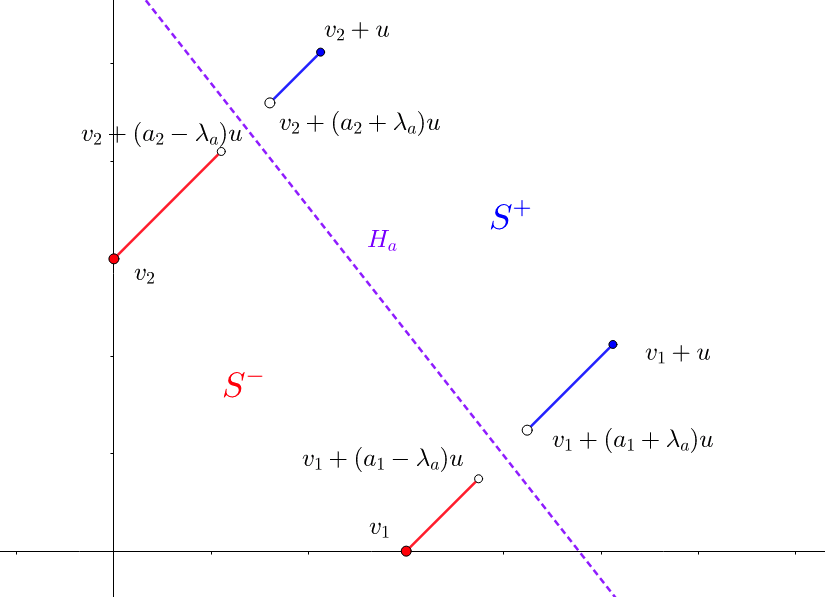
\includegraphics[scale=0.5]{d_a_pic}
\vspace{.3in}
\caption{An illustration of $\D_a$ in two dimensions. $S^-$ is shown in red, and $S^+$ is shown in blue. The decision boundary, $H_a$, of the optimal linear classifier, $f_{w^a, 1}$, is shown in purple. }
\label{fig:d_a_illustration}
\end{figure}

We include an example of such a distribution in Figure \ref{fig:d_a_illustration}. Next, we explicitly compute a linear classifier that linearly $r$-separates $\D_a$.

\begin{defn}\label{def:normal_vector}
Let $a \in [0,1]^d$, and let $\overline{a} = \sum_{i=1}^d a_i.$ Then let $w^a$ be defined as $$w_i^a = \frac{1}{\rr} - \frac{da_i}{\rr\sqrt{d} + d\rr\overline{a}}.$$ 
\end{defn}

\begin{lem}\label{lem:normal_vector_works}
$w^a$ satisfies $\langle w^a, u\rangle = \frac{d}{\sqrt{d} + d\overline{a}}$ and $\langle w^a, v_i + a_iu \rangle = 1,$ for all $1 \leq i \leq d.$ 
\end{lem}

\begin{proof}
By the definitions of $v_i, u$, we have that 
\begin{equation*}
\begin{split}
\langle w^a, u \rangle &= \langle w^a, \frac{1}{\sqrt{d}}\sum_1^d v_i \rangle \\
&= \frac{1}{\sqrt{d}} \sum_1^d Rw_i^a \\
&= \frac{1}{\sqrt{d}} \sum_1^d 1 - \frac{da_i}{\sqrt{d} + d\overline{a}} \\
&= \frac{1}{\sqrt{d}} \sum_1^d \frac{\sqrt{d} + d\overline{a} - da_i}{\sqrt{d} + d\overline{a}} \\
&= \frac{1}{\sqrt{d}} \frac{d\sqrt{d}}{\sqrt{d} + d\overline{a}} = \frac{d}{\sqrt{d} + d\overline{a}},
\end{split}
\end{equation*}
Which proves the first claim. Next, we also have that $\langle w^a, v_i \rangle = Rw_i^a$. Summing these, we get $$Rw_i^a + \frac{da_i}{\sqrt{d} + d\overline{a}} = 1 - \frac{da_i}{\sqrt{d} + d\overline{a}} + \frac{da_i}{\sqrt{d} + d\overline{a}} = 1,$$ as desired. 
\end{proof}

We now prove that $\D_a$ is linearly $r$-separated.

\begin{lem}\label{lem:separation}
$\D_a$ is linearly $r$-separated by the classifier $f_{w_a, 1}$.
\end{lem}

\begin{proof}
Let $H_a$ denote the hyperplane passing through $\{v_i + a_iu: 1 \leq i \leq d\}$. By Lemma \ref{lem:normal_vector_works}, $H_a$ is the decision boundary of $f_{w_a, 1}$.  Referring to Figure \ref{fig:d_a_illustration}, we see that $\cup S^+$ lies entirely above $H_a$ while the set $\cup S^-$ lies entirely below the hyperplane $H_a$, which the classifier $f_{w^a, 1}$ has accuracy $1$ with respect to $\D_a$. It suffices to show that $f_{w^a, 1}$ is robust everywhere. In order to do this, we must show that all points in the support of $\D_a$ have $\ell_p$ distance at least $r$ from $H_a$. 

Fix any $1 \leq i \leq d$. Since the $\ell_p$ distance metric is invariant under translation and scales linearly with dilations, it follows that the point $x_i = v_i + (a_i - \lambda_a)u$ is the closest point on the segment $[v_i, v_i+(a_i - \lambda_a)u)$ to $H_a$. Suppose $x_i$ has distance $D$ under the $\ell_p$ norm to $H_a$. Then the key observation is that the $\ell_p$ ball, $B_p(x_i, D)$, must be tangent to $H_a$. Expressing this as an equation, we have $\max_{z \in B_p(x_i, D)} \langle z, w^a \rangle = 1,$ which can be re-written as $$\max_{||z - x_i||_p \leq D} \langle z - x_i, w^a \rangle = 1 - \langle x_i, w^a \rangle.$$ By Lemma \ref{lem:normal_vector_works} , $\langle w^a, u \rangle = \frac{d}{\sqrt{d} + d\overline{a}}$ and $\langle w^a, v_i + a_iu \rangle = 1$. Substituting this, we see that 
\begin{equation*}
\begin{split}
1 - \langle x_i, w^a \rangle &= 1 - \langle v_i + a_iu - \lambda_a u, w^a \rangle \\
&= 1 - \langle v_i + a_iu, w^a \rangle + \langle \lambda_a u, w^a \rangle \\
&= \langle \lambda_a u, w^a \rangle \\
&= \frac{d\lambda_a}{\sqrt{d} + d\overline{a}}.
\end{split}
\end{equation*}

However, by using the dual norm, we see that $\max_{||z - x_i||_p \leq D} \langle z - x_i, w^a \rangle = D||w^a||_q$. Thus it follows that
\begin{equation*}
\begin{split}
D &= \frac{d\lambda_a}{(\sqrt{d} + d\overline{a})||w^a||_q} \\
&= \frac{d\frac{r}{\rr}f_q(a)}{(\sqrt{d} + d\overline{a})||w^a||_q} \\
&= \frac{d\frac{r}{\rr}\sqrt[q]{\sum_1^d |\frac{1}{\sqrt{d}} + \overline{a} - a_i|^q}}{(\sqrt{d} + d\overline{a})||w^a||_q} \\
&= \frac{r\sqrt[q]{\sum_1^d |\frac{1}{\rr}\frac{\sqrt{d} + d\overline{a} - da_i}{(\sqrt{d} + d\overline{a})}|^q}}{||w^a||_q} \\
&= \frac{r||w^a||_q}{||w^a||_q} = r.
\end{split}
\end{equation*}
We can use an analogous argument holds for $v_i + (a_i + r_a)u$, the closest point to $H_a$ in $S^+$. Thus each point in the support of $D^a$ has distance strictly larger than $r$ (as the endpoints were not included) to $H_a$. Consequently $f_{w^a, 1}$ linearly $r$-separates $D^a$, as desired. 
\end{proof}

\subsubsection{Defining $\dd$}\label{subsubsec:dd}

Now that we have defined $\D_a$, we turn our attention to defining $\A$, which requires us to specify a distribution over valid choices of $a$. In particular, although $\D_a$ is defined for $a \in [0, 1]^d$, we will require a more stringent condition on $a$ for our construction to work. To this end, we begin by defining $\Delta$, a key parameter that characterizes the domain of $a$. To define $\dd$, we use the following lemma.

\begin{lem}\label{lem:dd}
There exists a real number $\dd > 0$ such that for all $l \in \{2, q\}$, and for all $a \in [\frac{1}{2} - \dd, \frac{1}{2} + \dd]^d$, $$||\nabla f_l(a)||_2 \leq \frac{1}{d^2\sqrt{d}},$$ where $f_l$ is as defined in Definition \ref{defn:function_f}.
\end{lem}

\begin{proof}
Since $1 \leq q < \infty$, we see that for both choices of $l$, the function $h_l(x) = (\frac{1}{\sqrt{d}} - x)^l$ is a convex function for $x \in [-\frac{1}{2\sqrt{d}}, \frac{1}{2\sqrt{d}}]$. Thus, if $\sum_1^d x_i = 0$, then by Jensen's inequality, $\sum_1^d h_l(x_i) \geq \sum_1^d h_l(0)$. Applying this, we see that for all $l \in \{2, q\}$ and for all $a \in [\frac{1}{2} - \frac{1}{4\sqrt{d}}, \frac{1}{2} + \frac{1}{4\sqrt{d}}]^d$, 
\begin{equation*}
\begin{split}
f_l(a) &= \sqrt[l]{\sum_1^d |\frac{1}{\sqrt{d}} + \overline{a} - a_i|^l} \\
&= \sqrt[l]{\sum_1^d \left(\frac{1}{\sqrt{d}} + \overline{a} - a_i\right)^l} \\
&= \sqrt[l]{\sum_1^d h_l(a_i - \overline{a})} \\
&\geq \sqrt[l]{\sum_1^d h_l(0)} \\
&= f_l((\frac{1}{2}, \frac{1}{2}, \dots, \frac{1}{2})),
\end{split}
\end{equation*}
with the first equality holding since $\overline{a} - a_i < \frac{1}{\sqrt{d}}$ and the first inequality holding since $\sum_1^d a_i - \overline{a} = 0$. Thus $f_l(a)$ must be locally minimized when $a = (\frac{1}{2}, \frac{1}{2}, \dots, \frac{1}{2})$, and it follows that $$||\nabla f_l(\frac{1}{2}, \frac{1}{2}, \dots, \frac{1}{2})||_2 = 0, \text{ for } l = 2, q.$$ Now observe that the map $H(a) = \max_{l \in \{2, q\}} ||\nabla f_l(a)||_2$ is a continuous map as long as $|a_i - \overline{a}| < \frac{1}{\sqrt{d}}$ for all $1 \leq i \leq d$. Thus there exists an open neighborhood $U$ about $(\frac{1}{2}, \frac{1}{2}, \dots, \frac{1}{2})$ such that $H(a) \leq \frac{1}{d^2\sqrt{d}}$ for all $a \in U$. Taking $\dd$ so that $[\frac{1}{2} - \dd, \frac{1}{2} + \dd]^d \subseteq U$ suffices. 
\end{proof}

\begin{defn}\label{defn:Delta}
Let $\Delta$ be any constant for which Lemma \ref{lem:dd} holds. In particular, $\Delta$ only depends on $\ell_p$, the robustness norm, and $d$, the dimension.
\end{defn}

\subsubsection{Defining $\g_1$ and $\g_2$}\label{subsubsec:g1g2}

In this section, we define functions $\g_1, \g_2: [0, \frac{\Delta}{3}] \to [0, \frac{\Delta}{3}]$ which we will use to specify $\A$. Before defining $\g_1$ and $\g_2$, we will first prove several technical lemmas.

\begin{lem}\label{lem:phi_s}
Let $I \subseteq \R$ be an interval, and $\Phi:I \to \R$ be a strictly convex function.  For any $s \in \R$ and $t \geq 0$, let $\Phi_s(t) = \Phi(s-t) + \Phi(s + t)$. Then $\Phi_s$ is a strictly increasing function.
\end{lem}

\begin{proof}
Fix $s$, and let $0 \leq t_1 < t_2$. Then we see that by Jensen's inequality (for strictly convex functions), $$\Phi(s + t_1) < \frac{(t_2-t_1)\Phi(s+t_2)}{t_1 + t_2} + \frac{2t_1\Phi(s-t_1)}{t_1 + t_2},$$ and $$\Phi(s - t_1) < \frac{(t_2-t_1)\Phi(s-t_2)}{t_1 + t_2} + \frac{2t_1\Phi(s+t_1)}{t_1 + t_2}.$$ Summing these inequalities, we see that 
\begin{equation*}
\begin{split}
\Phi_s(t_1) &= \Phi(s - t_1) + \Phi(s + t_1) \\
&< \frac{(t_2-t_1)\Phi(s+t_2)}{t_1 + t_2} + \frac{2t_1\Phi(s-t_1)}{t_1 + t_2} + \frac{(t_2-t_1)\Phi(s-t_2)}{t_1 + t_2} + \frac{2t_1\Phi(s+t_1)}{t_1 + t_2} \\
&= \frac{t_2 - t_1}{t_1 + t_2}(\Phi(s +t_2) + \Phi(s - t_2)) + \frac{2t_1}{t_1 + t_2}(\Phi(s - t_1) + \Phi(s + t_1)) \\
&= \frac{t_2 - t_1}{t_1 + t_2}\Phi_s(t_2) + \frac{2t_1}{t_1 + t_2}\Phi_s(t_1).
\end{split}
\end{equation*}
Rearranging this yields $\Phi_s(t_1) < \Phi_s(t_2)$, as desired.
\end{proof}

\begin{lem}\label{lem:lipschitz}
Let $I \subseteq \R$ be an interval, $\Phi:I \to \R$ be a strictly convex continuous function, and  $x, y, z \in I$ be real numbers with $x < y < z$. Let $\epsilon >0$ be such that $x - \epsilon \in I$ and $y + \epsilon \leq z - \epsilon$. Then there exist unique $\delta, \gamma >0$ such that the following hold: $$\delta + \gamma = \epsilon,$$ $$\Phi(x-\delta) + \Phi(y + \epsilon) + \Phi(z - \gamma) = \Phi(x) + \Phi(y) + \Phi(z)$$
\end{lem}

\begin{proof}
Fix any $\epsilon$ satisfying the desired conditions, and define $\Theta: [0, \epsilon] \to \R$ as $\Theta(t) = \Phi(x - t) + \Phi(y + \epsilon) + \Phi(z + t - \epsilon)$. Then, utilizing the definition of $\Phi_s$ from Lemma \ref{lem:phi_s}, we see that $$\Theta(t) = \Phi_{\frac{x + z - \epsilon}{2}}(\frac{z - x - \epsilon}{2} + t) + \Phi(y + \epsilon).$$ By Lemma \ref{lem:phi_s}, it follows that $\Theta$ is strictly increasing in $t$, and since $\Phi$ is continuous, so is $\Theta$. Next, we bound $\Theta(0)$ and $\Theta(\epsilon)$ to put us in the configuration to apply the intermediate value theorem. To bound $\Theta(0)$, we have
\begin{equation*}
\begin{split}
\Theta(0) &= \Phi(x) + \Phi(y + \epsilon) + \Phi(z - \epsilon) \\
&= \Phi(x) + \Phi_{\frac{y+z}{2}}(\frac{z - y}{2} - \epsilon) \\
&< \Phi(x) + \Phi_{\frac{y+z}{2}}(\frac{z - y}{2}) \\
&= \Phi(x) + \Phi(y) + \Phi(z),
\end{split}
\end{equation*}
and to bound $\Theta(\epsilon)$, we have 
\begin{equation*}
\begin{split}
\Theta(\epsilon) &= \Phi(x - \epsilon) + \Phi(y + \epsilon) + \Phi(z) \\
&= \Phi_{\frac{x+y}{2}}(\frac{y- x}{2} + \epsilon) + \Phi(z)\\
&> \Phi_{\frac{x+y}{2}}(\frac{y - x}{2}) + \Phi(z) \\
&= \Phi(x) + \Phi(y) + \Phi(z).
\end{split}
\end{equation*}
Together, these equations imply $\Theta(0) < \Phi(x) + \Phi(y) + \Phi(z) < \Theta(\epsilon)$. Since $\Theta$ is strictly increasing and continuous, there exists a unique $\delta \in [0, \epsilon]$ such that $\Theta(\delta) = \Phi(x) + \Phi(y) + \Phi(z)$. Setting $\gamma = \epsilon - \delta$, we see that $$\Theta(\delta) = \Phi(x - \delta) + \Phi(y + \epsilon) + \Phi(z - \gamma) = \Phi(x) + \Phi(y) + \Phi(z),$$ as desired.


\end{proof}



Next, we define a function that will be useful for simplifying notation, both in this section and subsequent ones.

\begin{defn}\label{defn:F_the_function}
Let $\Delta$ be as in definition \ref{defn:Delta}. For $x, y, z \in [0, \frac{\dd}{3}]$, let $$F(x, y, z) = \sqrt[q]{\left(\frac{1}{\sqrt{d}} - x\right)^q + \left(\frac{1}{\sqrt{d}} - \frac{2\Delta}{3} + y\right)^q + \left(\frac{1}{\sqrt{d}} + \frac{2\Delta}{3} + z\right)^q}.$$
\end{defn}

We now define $\g_1, \g_2$.
\begin{cor}\label{cor:lipschitz_maps}
Let $\Delta$ be as in definition \ref{defn:Delta}. There exist $1$-Lipshitz, monotonically non-decreasing functions $\g_1, \g_2: [0, \frac{\dd}{3}] \to [0, \frac{\dd}{3}]$ such that for all $t \in [0, \frac{\dd}{3}]$, $\g_1(t) + \g_2(t) = t$ and $F(t, \g_1(t), \g_2(t)) = F(0, 0, 0)$. 
\end{cor}
\begin{proof}
We have two cases.
\paragraph{Case 1: $1 < q < \infty$:} Let $\Phi: [-\Delta, \Delta] \to \R$ be defined as $\Phi(x) = (\frac{1}{\sqrt{d}} - x)^q$. Since $q > 1$, and $\Delta < \frac{1}{\sqrt{d}}$, $\Phi$ is strictly convex. Observe that $$F(x, y, z)^q = \Phi(x) + \Phi(2\frac{\dd}{3} - y) + \Phi(-2\frac{\dd}{3} - z).$$ Next, fix any $t \in [0, \frac{\Delta}{3}]$. Then observe that $-\frac{2\Delta}{3} \geq -\Delta$ and that $\frac{2\Delta}{3} - t \geq 0 + t$. This puts us in the configuration to apply Lemma \ref{lem:lipschitz}. In particular, there exist unique reals $\delta_t, \gamma_t > 0$ such that $$\delta_t + \gamma_t = t,$$ $$\Phi(-\frac{2\Delta}{3} - \delta_t) + \Phi(t) + \Phi(\frac{2\Delta}{3} - \gamma_t) = \Phi(-\frac{2\Delta}{3}) + \Phi(0) + \Phi(\frac{2\Delta}{3}).$$ We now define $g_1, g_2: [0, \frac{\Delta}{3}] \to [0, \frac{\Delta}{3}]$ as $$g_1(t) = \gamma_t\text{ and }g_2(t) = \delta_t.$$ Then it is clear that $F(0,0,0) = F(t, g_1(t), g_2(t))$ and $g_1(t) + g_2(t)$ (by directly substituting into the equations above). All that remains is to show that $g_1$ and $g_2$ are 1-Lipschitz. 

Fix any $0 \leq t_1 < t_2 \leq \frac{\Delta}{3}$, and let $t_2 - t_1 = \epsilon$. The key idea is to apply Lemma \ref{lem:lipschitz} to $-\frac{2\Delta}{3} - g_2(t_1)<  t_1 < \frac{2\Delta}{3} - g_1(t_1)$ and $\epsilon$. To do so, we first check the conditions of the lemma. 

We have that $$-\frac{2\Delta}{3} - g_2(t_1) - \epsilon \geq -\frac{2\Delta}{3} - t_1 - \epsilon = -\frac{2\Delta}{3} - t_2 \geq -\Delta,$$ and 
\begin{equation*}
\begin{split}
t_1 + \epsilon &= t_2 \\
&\leq \frac{\Delta}{3} \\
&\leq \frac{2\Delta}{3} - t_2 \\
&= \frac{2\Delta}{3} - t_1 - \epsilon \\
&\leq \frac{2\Delta}{3} - g_1(t_1) - \epsilon.
\end{split}
\end{equation*}

Thus $\epsilon$ satisfies the necessary conditions for Lemma \ref{lem:lipschitz}. Since $\Phi$ is strictly convex, by Lemma \ref{lem:lipschitz}, there exist unique $\delta, \gamma > 0$ with $\delta+ \gamma = \epsilon$ such that $$\Phi(-\frac{2\Delta}{3} - g_2(t_1) - \delta) + \Phi(t_1 + \epsilon) + \Phi(\frac{2\Delta}{3} - g_1(t_1) - \gamma) = \Phi(-\frac{2\Delta}{3} - g_2(t_1)) + \Phi(t_1) + \Phi(\frac{2\Delta}{3} - g_1(t_1)).$$ However, by the definition of $g_1, g_2$, we see that both of these quantities are equal to $F(0,0,0)^q$. Moreover, again by the definition of $g_1, g_2$, we also have that $g_1(t_2)$ and $g_2(t_2)$ are the unique real numbers in $[0, \frac{\Delta}{3}$ that satisfy $$\Phi(-\frac{2\Delta}{3} - g_2(t_2)) + \Phi(t_2) + \Phi(\frac{2\Delta}{3}+g_1(t_2)) = F(0,0,0)^q.$$ Thus, it follows that $g_2(t_2) = g_2(t_1) + \delta$ and $g_1(t_2) = g_1(t_1) + \gamma$. However, $t_2 - t_1 = \epsilon$, and $\delta, \gamma < \epsilon$ (since they sum to $\epsilon$). Thus, we see that $|g_1(t_2) - g_1(t_1)| \leq |t_2 - t_1|$ and $|g_2(t_2) - g_2(t_1)| \leq |t_2 - t_1|$. Since $t_1$ and $t_2$ were arbitrary, it follows that $g_1$ and $g_2$ are both $1$-Lipschitz, as desired. 

Finally, since $\delta, \gamma > 0$, it follows that $g_2(t_2) > g_2(t_1)$ and $g_1(t_2) > g_1(t_1)$. Since $t_1, t_2$ were arbitrary, it follows that $g_1, g_2$ are monotonically non-decreasing.

\paragraph{Case 2: $q = 1$} In this case, since $\Delta < \frac{1}{\sqrt{d}}$ (Lemma \ref{lem:dd}), we see that $F(x, y, z) = \frac{3}{\sqrt{d}} + y + z - x$. Setting $\g_1(t) = \g_2(t) = \frac{t}{2}$ suffices, and clearly satisfies the desired properties. 
\end{proof}

\begin{defn}\label{defn:g_1_and_g_2}
Let $\Delta$ be as defined in Definition \ref{defn:Delta}. We let $g_1, g_2: [0, \frac{\Delta}{3}] \to [0, \frac{\Delta}{3}]$ be defined as any function satisfying the conditions of Corollary \ref{cor:lipschitz_maps}.
\end{defn}

\subsubsection{Putting it all together: defining $\A$}\label{subsubsec:finalA}

We are now ready to define $\A$. For convenience, we assume $d$ is a multiple of $3$.
\begin{defn}\label{defn:A}
Let $\Delta, g_1$, and $g_2$ be as defined in Definitions \ref{defn:Delta} and \ref{defn:g_1_and_g_2}. Then $\A$ is defined as the distribution of distributions $\D_a$ where $a$ is a random vector constructed as follows. Let $t_1, t_2, \dots t_{d/3}$ be drawn i.i.d from the uniform distribution over $[0, \frac{\dd}{3}]$. Then for $1 \leq i \leq d/3$, we let
	\begin{itemize}
		\item $a_i = \frac{1}{2} + t_i$.
		\item $a_{i+d/3} = \frac{1}{2} + 2\frac{\dd}{3} - g_1(t_i)$.
		\item $a_{i + 2d/3} = \frac{1}{2} - 2\frac{\dd}{3} - g_2(t_i).$
	\end{itemize}
Together the variables $a_1, a_2, \dots, a_d$ compose $a$. Thus a random distribution $\D \sim \A$ can be constructed by sampling $a$ as above and setting $\D = \D_a$.
\end{defn}

We now show that for all $\D_a \sim \A$, $\lambda_a$ (Definition \ref{def:w_dist}) is constant.

\begin{lem}\label{lem:cons_lambda}
There exists a constant $\Lambda$ such that for all $\D_a \sim \A$, $\lambda_a = \Lambda$. 
\end{lem}

\begin{proof}
Let $\D_a \sim \A$ be arbitrary. By Lemma \ref{cor:lipschitz_maps}, for all $1 \leq i \leq d$, $g_1(t_i) + g_2(t_i) = t_i$. Substituting this, we see that 
\begin{equation*}
\begin{split}
\overline{a} &= \frac{1}{d}\sum_1^d a_i \\
&= \frac{1}{d}\sum_1^{d/3} (\frac{1}{2} + t_i) + (\frac{1}{2} + \frac{2\Delta}{3} - g_1(t_i)) + (\frac{1}{2} - \frac{2\Delta}{3} - g_2(t_i)) \\
&= \frac{1}{d}\sum_1^{d/3} \frac{3}{2} \\
&= \frac{1}{2}.
\end{split}
\end{equation*}

Recall that $\lambda_a = \frac{r}{R}f_q(a) = \frac{r}{R}\sqrt[q]{\sum_1^d |\frac{1}{\sqrt{d}} + \overline{a} - a_i|^q}$. By substituting that $\overline{a} = \frac{1}{2}$ and expressing each $a_i$ in terms of $t_i$, we see that 
\begin{equation*}
\begin{split}
\lambda_a &=  \frac{r}{R}\sqrt[q]{\sum_1^d |\frac{1}{\sqrt{d}} + \overline{a} - a_i|^q}\\
&= \frac{r}{R}\sqrt[q]{\sum_{i=1}^{d/3} \left|\frac{1}{\sqrt{d}} + \frac{1}{2} - (\frac{1}{2} + t_i)\right|^q + \left|\frac{1}{\sqrt{d}} + \frac{1}{2} - \left(\frac{1}{2} + \frac{2\Delta}{3} - g_1(t_i)\right)\right|^q +  \left|\frac{1}{\sqrt{d}} + \frac{1}{2} - \left(\frac{1}{2} - \frac{2\Delta}{3} - g_2(t_i)\right)\right|^q} \\
 &= \frac{r}{R}\sqrt[q]{\sum_1^{d/3} \left|\frac{1}{\sqrt{d}} - t_i\right|^q + \left|\frac{1}{\sqrt{d}} + g_1(t_i) - \frac{2\Delta}{3}\right|^q + \left|\frac{1}{\sqrt{d}} + g_2(t_i) + \frac{2\Delta}{3}\right|^q} \\
&= \frac{r}{R}\sqrt[q]{\sum_1^{d/3}F(t_i, g_1(t_i), g_2(t_i))^q}, \\
\end{split}
\end{equation*}
where $F$ is defined as in Definition \ref{defn:F_the_function}. Next, by Corollary \ref{cor:lipschitz_maps}, $F(t_i, g_1(t_i), g_2(t_i)) = F(0,0,0)$ for all $1 \leq i \leq \frac{d}{3}$. Thus, if we set $\Lambda = \frac{r}{R}(\frac{d}{3})^{1/q}F(0,0,0)$, we have 
\begin{equation*}
\begin{split}
\lambda_a &= \frac{r}{R}\sqrt[q]{\sum_1^{d/3} F(t_i, g_1(t_i), g_2(t_i))^q} \\
&= \frac{r}{R}\sqrt[q]{\sum_1^{d/3}F(0,0,0)^q} \\
&= \frac{r}{R}\sqrt[q]{\frac{d}{3}F(0,0,0)^q} \\
&=  \frac{r}{R}(\frac{d}{3})^{1/q}F(0,0,0) = \Lambda,
\end{split}
\end{equation*}
proving the claim.
\end{proof}

\begin{defn}\label{defn:big_lambda}
We define $\Lambda = \frac{r}{R}(\frac{d}{3})^{1/q}F(0,0,0)$, where $F$ is defined as in Definition \ref{defn:F_the_function}.
\end{defn}

Next, we compute upper and lower bounds on $\Lambda$, both of which will be useful for subsequent lemmas. 
\begin{lem}\label{lem:lambda_bounds}
$\frac{1}{9} < \Lambda < \frac{1}{3}$. 
\end{lem}

\begin{proof}
By definition, $\Lambda = \frac{d}{3}^{1/q}F(0, 0, 0)$. Substituting the definition of $f$, we see that  $F(0, 0, 0) = \sqrt[q]{|\frac{1}{\sqrt{d}}|^q + |\frac{1}{\sqrt{d}} - \frac{2\Delta}{3}|^q + |\frac{1}{\sqrt{d}} + \frac{2\Delta}{3}|^q},$ and consequently, $$3^{1/q}|\frac{1}{\sqrt{d}} - \frac{2\Delta}{3}| \leq F(0, 0, 0) \leq 3^{1/q}|\frac{1}{\sqrt{d}} + \frac{2\Delta}{3}|.$$ By definition, $\frac{2\Delta}{3} < \frac{1}{2\sqrt{d}}$. It follows that $$\frac{r}{R}\frac{d^{1/q}}{2\sqrt{d}} < \Lambda < \frac{r}{R}\frac{3d^{1/q}}{2\sqrt{d}}.$$ Finally, since $\frac{r}{R} = \frac{2\sqrt{d}}{9d^{1/q}}$, substituting this yields $\frac{1}{9} < \Lambda < \frac{1}{3}$, as desired.
\end{proof}

Next, we show that for all $\D_a \in \A$, the aspect ratio (Definition \ref{defn:aspect_ratio}), $\rho(\D_a)$, is bounded by a constant.

\begin{lem}\label{lem:large_margin}
For all $\D_a \in \A$, we have $\rho(\D_a) \leq 18\sqrt{3}$. 
\end{lem}

\begin{proof}
We first bound the $\ell_2$ margin, $\gamma(\D_a)$ (Definition \ref{defn:margin}). Recall that the margin, $\gamma(\D_a)$ is described as the largest possible $\ell_2$ distance from the support of $\D_a$ to the decision boundary of a linear classifier. Thus, we can lower bound $\gamma(\D_a)$ by computing the distance from the support of $\D_a$ to $H_a$, the decision boundary of $f_{w^a, 1}$ (Definition \ref{def:normal_vector}).

By referring to Figure \ref{fig:d_a_illustration} (in Section \ref{subsubsec:D_a}), it becomes clear that the closest point (under the $\ell_2$ margin) from $S^-$ to $H_a$ is the point $v_i + (a_i - \lambda_a)u$, for some value of $i$. Thus it suffices to compute the $\ell_2$ distance from this point to the plane $H_a$. 

Recall that by Lemma \ref{lem:normal_vector_works}, the point $v_i + a_iu$ satisfies $\langle w^a, v_i + a_iu \rangle = 1$, and consequently must lie on the hyperplane $H_a$. Let $D$ denote the $\ell_2$ distance from $v_i + (a_i - \lambda_a)u$ to $H_a$. Since $w^a$ is the normal vector to $H_a$, it follows that
\begin{equation*}
\begin{split}
D &= \langle v_i + a_iu - (v_i + (a_i - \lambda_a)u), \frac{w^a}{||w^a||_2} \rangle \\
&= \frac{\langle \lambda_a u, w^a \rangle}{||w^a||_2} \\
&\numeq{1} \frac{\langle \Lambda u, w^a \rangle}{||w^a||_2} \\
&\numeq{2} \frac{\Lambda \frac{d}{\sqrt{d} + d\overline{a}}}{||w^a||_2}  \\
&\numeq{3} \frac{\Lambda \frac{d}{\sqrt{d} + d\overline{a}}}{\sqrt{\sum_1^d \left(\frac{\sqrt{d} + d\overline{a} - da_i}{R(\sqrt{d} + d\overline{a}}\right)^2}} \\
&= \frac{R\Lambda}{\sqrt{\sum_1^d (\frac{1}{\sqrt{d}} + \overline{a} - a_i)^2}} \\
&\numeq{4} \frac{R\Lambda}{f_2(a)}.
\end{split}
\end{equation*}
Here, (1) holds by Lemma \ref{lem:cons_lambda}, (2) holds by Lemma \ref{lem:normal_vector_works}, (3) holds by Definition \ref{def:normal_vector}, and (4) holds by Definition \ref{defn:function_f}.

Next, observe that since $\D_a \sim \A$, we must have $a \in [\frac{1}{2} - \Delta, \frac{1}{2} + \Delta]^d$. Thus it follows that $||a - (\frac{1}{2}, \frac{1}{2}, \dots, \frac{1}{2})||_2 \leq \Delta\sqrt{d}$. However, by applying Lemma \ref{lem:dd}, we also see that $f_2$ is $\frac{1}{d^2\sqrt{d}}$-Lipschitz over $[\frac{1}{2} - \Delta, \frac{1}{2} + \Delta]^d$. Thus, it follows that $$f_2(a) \leq f_2(\frac{1}{2}, \frac{1}{2}, \dots, \frac{1}{2}) + \Delta\sqrt{d} \frac{1}{d^2\sqrt{d}} \leq 2,$$ with the latter inequality holding from the definition of $\Delta$. 

Substituting this and applying Lemma \ref{lem:lambda_bounds}, we see that $$\gamma(\D_a) \geq \frac{R\Lambda}{2} \geq \frac{R}{18}.$$ Next, to bound the aspect ratio, $\rho(\D_a)$, we must also bound the $\ell_2$ diameter of $\D_a$. However, the $\ell_s$ diameter of $\D_a$ is $R\sqrt{3}$, since it is the distance from $v_i + u$ to $v_j$ for $i \neq j$. Thus, it follows that $$\rho(\D_a) = \frac{diam_2(\D_a)}{\gamma(\D_a)} \leq \frac{R\sqrt{3}}{R/18} = 18\sqrt{3},$$ as desired. 
\end{proof}

Note that a tighter analysis (and selection of $\Delta$) can give a smaller bound for $\rho(\D_a)$, but the most important fact is that $\rho(\D_a) = O(1)$. 

\subsection{Bounding the expected robust loss}\label{subsec:bound_expectation}

In this section, we finally prove our lower bound, Theorem \ref{thm:lower}. This will require a few important steps, which we have separated into the following subsections. 
\begin{itemize}
	\item In section \ref{subsubsec:loss_bounding}, we give a useful lower bound for the loss $\L_r(f, \D_a)$ where $f$ is an arbitrary linear classifier. 
	\item In section \ref{subsubsec:posterior}, we give an explicit computation for the posterior distribution $\A|S$ where $S \sim \D_a^n$ is the observed training sample. 
	\item Finally, in section \ref{subsubsec:proof}, we present the proof of Theorem \ref{thm:lower}.
\end{itemize}

\subsubsection{Bounding the loss $\L_r(f, \D_a)$}\label{subsubsec:loss_bounding}

In this section, we find a lower bound on the loss $\L_r(f, \D_a)$ where $f$ is a linear classifier. We begin by first restricting $f$ to be in the set of classifiers $$f \in \{f_{w^b, 1}: b \in [0, 1]^d\},$$ where $w^b$ is as defined in Definition \ref{def:normal_vector}. These are precisely the classifiers that have a decision boundary that passes through some point on every line segment in $\{[v_i, v_i + u]: 1 \leq i \leq d\}$. We are able to only consider these classifiers since all other linear classifiers clearly have a very high loss with respect to $\D_a$ as they necessarily misclassify at least half the points on the line segment $[v_i, v_i + u]$ for some value of $i$. 

We now find an initial lower bound on $\L_r(f_{w^b, 1}, \D_a)$.

\begin{lem}\label{lem:loss_bound_general}
Fix any $\D_a \in \A$, and let $b \in [0,1]^d$ be arbitrary. Let $w^b$ be the vector defined as in Definition \ref{def:normal_vector}, and $\lambda_b = \frac{r}{\rr}\f_q(b)$ where $f$ is as defined in Definition \ref{defn:function_f}. Then $$\L_r(f_{w^b, 1}, \D_a) \geq \frac{d(\lambda_b - \lambda_a) + \sum_1^d|a_i - b_i|}{d - 2d\Lambda}.$$ 
\end{lem}

\begin{proof}
By Lemma \ref{lem:separation}, $f_{w^b, 1}$ precisely $r$-separates $\D_b$. This implies that for all $1 \leq i \leq d$,
$$f_{w^b, 1}(x) = \begin{cases} 1 & x \in (v_i + (b_i + \lambda_b)u, v_i + u] \\-1 & x \in [v_i, v_i + (b_i - \lambda_b)u) \\ \text{not robust} & x \in [v_i + (b_i - \lambda_b)u, v_i + (b_i + \lambda_b)u] \end{cases}.$$ Without loss of generality, suppose that $b_i \geq a_i$. The key observation is that for all $1 \leq i \leq d$, if $x \in [v_i + (a_i + \lambda_a)u, v_i + (b_i + \lambda_b)u]$, then $f_{w^b, 1}(x) = -1$ for $f_{w^b, 1}$ is not robust at $x$. In both cases, we see that $f_{w^b, 1}$ is either inaccurate or not robust for all points in $[v_i + (a_i + \lambda_a)u, v_i + (b_i + \lambda_b)u]$. 

This interval has $\ell_2$ length at least $(|a_i - b_i| + (\lambda_b - \lambda_a))||u||_2$. Note that in the case that $a_i \leq b_i$ we can get an identical expression. Thus,  combining this for all $i$, we see that $f_{w^b, 1}$ is either inaccurate or not robust for a total length of $[d(\lambda_b - \lambda_a) + \sum_1^d |a_i - b_i|]||u||_2$. Dividing by the total length of the support of $\D_a$, we find that
\begin{equation*}
\begin{split}
\L_r(f_{w^b, 1}, \D_a) &\geq \frac{[d(\lambda_b - \lambda_a) + \sum_1^d |a_i - b_i|]||u||_2}{\sum_1^d ||[v_i, v_i + (a_i - \lambda_a)u) + (v_i + (a_i + \lambda_a)u, v_i + u]||_2} \\
&= \frac{[d(\lambda_b - \lambda_a) + \sum_1^d |a_i - b_i|]||u||_2}{\sum_1^d ||u_2||(1 - 2\lambda_a)} \\
&= \frac{d(\lambda_b - \lambda_a) + \sum_1^d |a_i - b_i|}{d(1 - 2\lambda_a)} \\
&= \frac{d(\lambda_b - \lambda_a) + \sum_1^d |a_i - b_i|}{d - 2d\Lambda},
\end{split}
\end{equation*}
with the last equality holding since by Lemma \ref{lem:cons_lambda}, $\lambda_a = \Lambda$. 
\end{proof}

\begin{lem}\label{lem:loss_bound_clever}
For all $\D_a \in \A$ and $b \in [0,1]^d$, $d(\lambda_a - \lambda_b) \leq \frac{1}{2}\sum_1^d |a_i - b_i|.$ 
\end{lem}

\begin{proof}
We have two cases.
\paragraph{Case 1:} $b \in [\frac{1}{2} - \Delta, \frac{1}{2} + \Delta]^d$.

Observe that $\lambda_b = \frac{r}{R}f_q(b)$ and $\lambda_a = \frac{r}{R}f_q(a)$. By Lemma \ref{lem:dd}, we see that $f_q$ is $\frac{1}{d^2\sqrt{d}}$-Lipschitz over the domain $[\frac{1}{2} - \Delta, \frac{1}{2} + \Delta]^d$. It follows that
\begin{equation*}
\begin{split}
\lambda_a - \lambda_b &= \frac{r}{R}(f_q(a) - f_q(b)) \\
&\leq \frac{r}{R}||a - b||_2\frac{1}{d^2\sqrt{d}} \\
&= \frac{2\sqrt{d}}{9d^{1/q}}||a - b||_2\frac{1}{d^2\sqrt{d}} \\
&< \frac{||a - b||_1}{2d},
\end{split}
\end{equation*}
with the last inequality following since the $\ell_2$ norm is smaller than the $\ell_1$ norm. Rearranging this gives the statement of the Lemma as desired.

\paragraph{Case 2: } $b \notin [\frac{1}{2} - \Delta, \frac{1}{2} + \Delta]^d$.

The main idea in this case will be to find $b' \in [\frac{1}{2} - \Delta, \frac{1}{2} + \Delta]^d$ such that $\lambda_b \geq \lambda_{b'}$ and such that $||b' - a||_1 \leq ||b - a||_1$. We will then apply Case 1 to get the desired result.

Without loss of generality, assume that $b_1 \geq b_2 \geq \dots \geq b_d$, and that $b_1, b_2, \dots b_k > \frac{1}{2} + \Delta$, $b_{k+1}, \dots, b_l \in [\frac{1}{2} - \Delta, \frac{1}{2} + \Delta]$, and $b_{l+1}, \dots b_d < \frac{1}{2} - \Delta$ for some values of $k$ and $l$. 

We will construct $b'$ in four steps. In each of these steps, we will change the values of $b_i$ such that neither $||a - b||_1$ nor $\lambda_b$ are increased. At each step, we let $b_i$ refer to its value at the end of the previous step. 


Finally, for reference, recall that $$\lambda_b = \frac{r}{R}f_q(b) = \frac{r}{R}\sqrt[q]{\sum_1^d |\frac{1}{\sqrt{d}} + \overline{b} - b_i|^q}.$$

\paragraph{Step 1:} We set $$b_i \leftarrow  \begin{cases} \frac{1}{k}\sum_{j=1}^k b_j & 1 \leq i \leq k \\b_i & k+1 \leq i \leq l \\  \frac{1}{d-l}\sum_{j=l+1}^d b_j& l+1 \leq i \leq d \end{cases}.$$ Since $a \in [\frac{1}{2} - \Delta, \frac{1}{2} + \Delta]^d$, we see that these operations do not change $||a - b||_1$, as $\sum_1^k |b_i - a_i| = \sum_1^k b_i - a_i$ and $\sum_{l+1}^d |b_i - a_i| = \sum_1^k a_i - b_i$. Also, observe that this operation preserves $\overline{b}$, and consequently since the function $f(x) = |\frac{1}{\sqrt{d}} + \overline{b} - x|^q$ is convex, we see that by Jensen's inequality that $\lambda_b$ is not increased by this operation.

\paragraph{Step 2:} Let $\beta = \sum_1^k(b_i - \frac{1}{2} - \Delta) - \sum_{l+1}^d (\frac{1}{2} - \Delta - b_i)$. Then we set $$b_i \leftarrow  \begin{cases} \begin{cases} \frac{1}{2} + \Delta + \frac{\beta}{k} & 1 \leq i \leq k \\ b_i & k+1 \leq i \leq l \\ \frac{1}{2} - \Delta & l+1 \leq i \leq d \end{cases} & \beta \geq 0 \\\begin{cases} \frac{1}{2} + \Delta & 1 \leq i \leq k \\ b_i & k+1 \leq i \leq l \\ \frac{1}{2} - \Delta + \frac{\beta}{d - l} & l+1 \leq i \leq d \end{cases} & \beta < 0\end{cases}.$$

Observe that this operation cannot increase $||a - b||_1$, since it doesn't increase $|a_i - b_i|$ for any value of $i$. Furthermore, this operation also does not change $\overline{b}$, and a similar convexity argument on the function $f(x) = |\frac{1}{\sqrt{d}} + \overline{b} - x|^q$ can show that this does not increase $\lambda_b$. 

Finally, if $\beta = 0$, we set $b' = b$, since we have reached a state such that $b \in [\frac{1}{2} - \Delta, \frac{1}{2} + \Delta]^d$. 

\paragraph{Step 3a:} We run this step if $\beta > 0$. Let $\alpha = \frac{\sum_{k+1}^d (\frac{1}{2} + \Delta - b_i)}{\beta}$. We then set  $$b_i \leftarrow  \begin{cases} \begin{cases} \frac{1}{2} + \Delta & 1 \leq i \leq k \\ (\frac{1}{2} + \Delta)(\frac{\alpha - 1}{\alpha}) + \frac{b_i}{\alpha} & k+1 \leq i \leq d \end{cases} & \alpha \geq 1 \\\begin{cases} \frac{1}{2} + \Delta + \frac{\beta}{k}(1 - \alpha) & 1 \leq i \leq k \\ \frac{1}{2} + \Delta & k+1 \leq i \leq d \end{cases} & \alpha < 1\end{cases}.$$ In this step, we can similarly verify that $||a - b||_1$ does not increase (as $|a_i - b_i|$ is strictly reduced for $1 \leq i \leq k$ by an exact amount to offset the possible increases in $|a_i - b_i|$ for $k+1 \leq i \leq d$). We also see by the same convexity argument as usual that this operation reduces $\lambda_b$. 

\paragraph{Step 3b:} We run this step if $\beta < 0$. Let $\alpha = \frac{\sum_{k+1}^d (b_i - \frac{1}{2} + \Delta)}{\beta}$. We then set  $$b_i \leftarrow  \begin{cases} \begin{cases} (\frac{1}{2} - \Delta)(\frac{\alpha - 1}{\alpha}) + \frac{b_i}{
\alpha} & 1 \leq i \leq l \\ \frac{1}{2} - \Delta & k+1 \leq i \leq d \end{cases} & \alpha \geq 1 \\\begin{cases} \frac{1}{2} - \Delta & 1 \leq i \leq l \\ \frac{1}{2} - \Delta + \frac{\beta}{d-l}(1-\alpha) & l+1 \leq i \leq d \end{cases} & \alpha < 1\end{cases}.$$ The justification for this step is analogous to 3a.

\paragraph{Step 4:} We only run this step if $\alpha < 1$. Observe that if $\alpha \geq 1$, then both Step 3a and Step 3b result with $b \in [\frac{1}{2} - \Delta, \frac{1}{2} + \Delta]^d$, which we set as $b'$. Observe that in this case, either $b_i \geq a_i$ for all $i$, or $b_i \leq a_i$ for all $i$. Thus we simply set $$b_i \leftarrow \overline{b}.$$ This operation does not change $||a - b||_1$, and it also reduces $\lambda_b$ (by a convexity argument). 

\paragraph{Step 5:} Finally, for all $1 \leq i \leq d\Delta$, we set $b_i = \frac{1}{2}-\Delta$ if $\overline{b} < \frac{1}{2} - \Delta$ and otherwise set $b_i = \frac{1}{2} - \Delta$ if $\overline{b} > \frac{1}{2} + \Delta$. In both cases, $\lambda_b$ is not changed, and $||a-b||_1$ is strictly reduced. In this step, we finally set $b' = b$. Note that we do not always reach this step, as it was possible in any of the previous steps to reach some $b \in [\frac{1}{2} - \Delta, \frac{1}{2} + \Delta]^d$, at which point we would have simply terminated.

\paragraph{Conclusion: } Through steps $1$ through $5$, we have found $b' \in [\frac{1}{2} - \Delta, \frac{1}{2} + \Delta]^d$ such that $\lambda_{b'} \leq \lambda_b$ and $||a - b'||_1 \leq ||a - b||_1$. By applying Case 1 to $b'$, we see that $d(\lambda_a - \lambda_{b'}) \leq \frac{1}{2}||a - b'||_1$. Thus, we have that $$\frac{1}{2}||a - b||_1 \geq \frac{1}{2}||a - b'||_1 \geq d(\lambda_a - \lambda_{b'}) \geq d(\lambda_a - \lambda_b),$$ which implies the result by the transitive property.


\end{proof}

From the previous two lemmas, we immediately have the following:
\begin{cor}\label{cor:l_1distancebound}
For all $\D_a \in \A$ and $b \in [0,1]^d$, $$\L_r(f_{w^b, 1}, \D_a) \geq \frac{1}{2d}\sum_1^d |a_i - b_i|.$$
\end{cor}

\begin{proof}
We have that
\begin{equation*}
\begin{split}
\L_r(f_{w^b, 1}, \D_a) &\numgeq{a} \frac{d(\lambda_b - \lambda_a) + \sum_1^d|a_i - b_i|}{d - 2d\Lambda} \\
&\geq \frac{\sum_1^d|a_i - b_i| - d(\lambda_a - \lambda_b) + }{d} \\
&\numgeq{b} \frac{\sum_1^d|a_i - b_i| - \frac{1}{2}\sum_1^d |a_i - b_i|}{d} \\
&= \frac{1}{2d}\sum_1^d |a_i - b_i|,
\end{split}
\end{equation*}
where (a) holds by Lemma \ref{lem:loss_bound_general} and (b) holds by Lemma \ref{lem:loss_bound_clever}. 
\end{proof}

\subsubsection{Computing the posterior distribution, $\A|S$}\label{subsubsec:posterior}

Recall that our ultimate goal is to show that $$\E_{\D \sim \A}[\E_{S \sim \D^n}[ \L_r(A_S, \D)]] \geq \Omega(\frac{d}{n}),$$ where $A$ denotes any learning algorithm returning a linear classifier.  The main idea for showing this is to ``switch expectations" and realize that $$\E_{\D \sim \A}[\E_{S \sim \D^n} [\L_r(A_S, \D)]] = \E_{S \sim \B}[\E_{\D \sim \A|S}[\L_r(A_S, \D)]],$$ where $\A|S$ denotes the posterior distribution over $\A$ after observing $S$. In this section, we fully characterize the distribution $\A|S$, and prove several important properties about it.

Recall (Definition \ref{defn:A}) that $\D_a \sim \A$ is generated by first choosing $t_1, t_2, \dots, t_{d/3} \sim \U[0, \frac{\dd}{3}]$ i.i.d, and then letting $a = (a_1, a_2, \dots, a_d)$ be a function of $t = (t_1, \dots, t_{d/3})$. Thus, to compute the posterior $\A|S$, it suffices to focus on the posterior distribution of $t|S$ for any $1 \leq i \leq \frac{d}{3}$. We begin by first defining the likelihood of observing $S$ given that it is generated from parameter $t$.

\begin{defn}\label{defn:L(S|t)}
Let $S = \{(x_1, y_1), (x_2, y_2), \dots, (x_n, y_n)\}$ be any set of $n$ points in $\R^d \times \{\pm 1\}$, and let $t \in [0, \frac{\Delta}{3}]^{d/3}$ be a vector. Let $a \in [\frac{1}{2} - \Delta, \frac{1}{2} + \Delta]^d$ be defined as in Definition \ref{defn:A}. That is, let 
\begin{itemize}
	\item $a_i = \frac{1}{2} + t_i$.
	\item $a_{i + d/3} = \frac{1}{2} + \frac{2\Delta}{3} - g_1(t_i)$.
	\item $a_{i + 2d/3} = \frac{1}{2} - \frac{2\Delta}{3} - g_2(t_i)$. 
\end{itemize}
Then we define $L(S|t)$ as the likelihood of observing the set $S$ from $\D_a^n$. In particular, for any measurable region of points $R \subseteq (\R^d \times \{\pm 1\})^n$, we have that $$\mathbb{P}_{S \sim \D_a^n}[S \in R] = \int_{x \in R}L(x|t)dx.$$
\end{defn}

\begin{lem}\label{lem:binary}
Let $S \subset \R^d \times \{\pm 1\}$ be a set with $n$ points. Then for all $t \in [0, \frac{\dd}{3}]^{d/3}$, $$L(S|t) \in \left\{0, \left(\frac{1}{(d - 2\Lambda)||u||_2}\right)^n\right\},$$ where $\Lambda$ is as defined in Definition \ref{defn:big_lambda} and $L(S|t)$ is as defined in Definition \ref{defn:L(S|t)}. 
\end{lem}

\begin{proof}
Let $\D_a$ be an arbitrary distribution in $\A$. Observe that $\D_a$ is uniform over the set of all points in its support. Thus for every point in its support, we have that the likelihood $L(x|t)$ satisfies $L(x|t) = \frac{1}{(d - 2\Lambda)||u||_2}$. 

Taking the product of this over all points in $S$, we get the desired result. Note that if $S$ contains some point not in the support of $\D_a$, then the likelihood becomes $0$, since the likelihood of observing some point not in the support of $\D_a$ is $0$.
\end{proof}


\begin{defn}\label{defn:permissible_set}
For any dataset $S$, let $P_S$ denote the set of all ``permissible" $t$, that is $t \in [0, \frac{\dd}{3}]^d$ such that $L(S|t) \neq 0$. Formally, $$P_S = \{t: L(S|t) >0\}.$$
\end{defn}

We now fully characterize $P_S$ when $S$ is drawn from some $\D \sim \A$.

\begin{lem}\label{lem:intervals}
Fix $n > 0$. For all $\D \sim \A$ and $S \sim \D^n$, there exist intervals (possibly open, closed, half open) $I_1^S, I_2^S, \dots, I_{d/3}^S \subseteq [0, \frac{\dd}{3}]$ such that $P_S = \prod_1^{d/3} I_i^S$.
\end{lem}

\begin{proof}
Let $S = \{(x_1, y_1), (x_2, y_2), \dots, (x_n, y_n)\}$. Since $S \sim \D^n$, we see that for $1 \leq j \leq n$, $x_j$ must satisfy $x_j \in [v_i, v_i + u]$ for some $1 \leq j \leq d$. Using this, for $1 \leq i \leq d$ let $$s_i^- = \argmax_{\{x_j: x_j \in [v_i, v_i + u], y_j = -1\}} ||x_j - v_i||_2,$$ and $$s_i^+ = \argmax_{\{x_j: x_j \in [v_i, v_i + u], y_j = +1\}} ||x_j - (v_i+ u)||_2.$$ $s_i^-$ and $s_i^+$ can be thought of as the points from $S$ on segment $[v_i, v_i + u]$ that are closest to each other and labeled as $-$ and $+$ respectively. As a default, if no such points exist, we set $s_i^- = v_i$ and $s_i^+ = v_i + u$. 

Next, consider any $t \in [0, \frac{\Delta}{3}]^{d/3}$, let $a \in [\frac{1}{2} - \Delta, \frac{1}{2} + \Delta]^d$ be defined as in Definition \ref{defn:A}. That is, let 
\begin{itemize}
	\item $a_i = \frac{1}{2} + t_i$.
	\item $a_{i + d/3} = \frac{1}{2} + \frac{2\Delta}{3} - g_1(t_i)$.
	\item $a_{i + 2d/3} = \frac{1}{2} - \frac{2\Delta}{3} - g_2(t_i)$. 
\end{itemize}
The key idea of this lemma is that $t \in P_S$ (i.e. $L(S|t) > 0$) if and only if for all $1 \leq i \leq d$, $$[v_i + (a_i - \Lambda)u, v_i + (a_i + \Lambda)u] \subseteq (s_i^-, s_i^+).$$  To see this, observe that if the claim above holds, then we must have that $s_i^- \in [v_i, v_i + (a_i - \Lambda)u)$ and $s_i^+ \in (v_i + (a_i + \Lambda)u, v_i + u]$, and it consequently follows that all points in $S$ are elements of the support of $\D_a$ (Definition \ref{def:w_dist}), as all other points in $S$ are ``further" from the interval $[v_i + (a_i - \Lambda)u, v_i + (a_i + \Lambda)u]$ than the points $s_i^+$ and $s_i^-$. Conversely, if $L(S|t) > 0$, we must have that $S \subseteq supp(\D_a)$, which immediately translates to the statement above. Thus, it suffices to find all $t$ such that this condition holds.

To do this, observe that the interval $[v_i + (a_i - \Lambda)u, v_i + (a_i + \Lambda)u]$ is a line segment of length $2\Lambda||u||_2$ that is centered at the point $v_i + a_iu$. Thus, in order for this to be a sub-segment of $(s_i^-, s_i^+)$, we only need that $a_i$ satisfy $v_i + a_iu \in (s_i^- + \Lambda u, s_i^- - \Lambda u)$. This condition is equivalent to the condition that $a_i \in J_i^S$ for some open interval $J_i^S \subseteq [0, 1]$, where $J_i^S$ is only dependent on $s_i^-, s_i^+$ and $\Lambda$ (which is a constant). In summary, there exist interval $J_1^S, J_2^S, \dots, J_d^S$ such that $t \in P_S$ if and only if $a_i \in J_i^S$ for $1 \leq i \leq d$.

Finally, note that for $1 \leq i \leq d/3$, $a_i, a_{i+d/3}, a_{i + 2d/3}$ are all functions of $t_i$, and moreover these functions are $1$-lipschitz, and monotonic. As a consequence, by taking the intersections of the pre-images of these functions, we find that this condition holds if and only if $t_i \in I_i^S$ where $I_i^S$ is some interval that is a subset of $[0, \frac{\Delta}{3}]^{d/3}$. This proves the claim.
\end{proof}

\begin{cor}\label{cor:posterior}
For any $S \sim \D$ where $\D \sim \A$, let $I_i^S$ be defined as in Lemma \ref{lem:intervals} for $1 \leq i \leq d/3$. Then the posterior distribution $t|S$ is equal to the uniform distribution over the set $\prod_{1 \leq i \leq d/3} I_i^S$, where $t_i$ is sampled from $I_i^S$. 
\end{cor}

\begin{proof}
First, recall that our prior on $t$ is $\U([0, \frac{\Delta}{3}]^d)$, where $\U$ denotes the uniform distribution. By Lemma \ref{lem:binary}, we see that for all $t \in P_S$, $L(S|t) = \left(\frac{1}{(d - 2\Lambda)||u||_2}\right)^n$, and for all other $t$, $L(S|t) = 0$. Furthermore, by Lemma \ref{lem:intervals}, we see that $P_S = \prod_1^{1 \leq i \leq d/3} I_i^S$. Thus, applying Bayes rules gives the desired result. 
\end{proof}

We conclude this section by lower bounding the expected length of the interval $I_i^S$, denoted $\ell(I_i^S)$. 
\begin{lem}\label{lem:expected_length}
For an interval $(c, d) \subset \R$, we let its length, denoted $\ell((c,d))$ be defined as $\ell((c,d)) = d - c$. Then for $1 \leq k \leq d/3$, the expected length (taken over $\D_a \sim \A$ and $S \sim \D_a^n$) of the interval $I_k^S$ is at least $\Omega(\frac{d}{n})$. That is, $$\E_{\D_a \sim \A}\E_{S \sim \D_a^n}[\ell(I_k^S)]] \geq \Omega(\frac{d}{n}).$$
\end{lem}

\begin{proof}
Fix any $\D_{a^*} \sim \Pi$, and let $t^*$ denote the value of $t$ used to generate $a$ (as in Definition \ref{defn:A}). We will show that $\E_{S \sim \D_{a^*}^n}[\ell(I_k^S)]] \geq \Omega(\frac{d}{n}),$ for all $1 \leq k \leq d/3$. We begin by explicitly computing the interval $I_k^S$. 

Fix $1 \leq k \leq d/3$. Then $t_k* \in [0, \frac{\Delta}{3}]$. Assume that $t_k^* > 0$; we will handle the case $t_k^* = 0$ separately. Recall from the proof of Lemma \ref{lem:intervals} that for $1 \leq i \leq d$, we defined $$s_i^- = \argmax_{\{x_j: x_j \in [v_i, v_i + u], y_j = -1\}} ||x_j - v_i||_2,$$ and $$s_i^+ = \argmax_{\{x_j: x_j \in [v_i, v_i + u], y_j = +1\}} ||x_j - (v_i+ u)||_2.$$ for $1 \leq i \leq d$. 

Next let $t \in [0, \frac{\Delta}{3}]^{d/3}$ be a vector, and let $a \in [\frac{1}{2} - \Delta, \frac{1}{2} + \Delta]^d$ be defined as $a_k = \frac{1}{2} + t_k$, $a_{k + d/3} = \frac{1}{2} + \frac{2\Delta}{3} - g_1(t_k)$ and $a_{k + 2d/3} = \frac{1}{2} - \frac{2\Delta}{3} - g_2(t_k)$, for $1 \leq k \leq d/3$. Note that $g_1, g_2$ are the functions defined in Definition \ref{defn:g_1_and_g_2}.

As we argued in the proof of Lemma \ref{lem:intervals}, it then follows that $t_k \in I_k^S$ if and only if $$[v_i + (a_i - \Lambda)u, v_i + (a_i + \Lambda)u] \subseteq (s_i^-, s_i^+),$$ for $i = k, k+d/3, k+2d/3$. Finally, as we did in Lemma \ref{lem:intervals}, for each $1 \leq i \leq d$, we define intervals $J_i^S \subseteq [\frac{1}{2} - \Delta, \frac{1}{2} + \Delta]$ such that $a_i \in J_i^S$ if and only if $[v_i + (a_i - \Lambda)u, v_i + (a_i + \Lambda)u] \subseteq (s_i^-, s_i^+)$. 


We now have the following three claims.

\paragraph{Claim 1:} Let $\alpha = \min \left(\frac{||s_k^- -  (v_k + (a_k^* - \Lambda)u)||_2}{||u||_2}, t_k^*\right)$. If $t_k \in (t_k^* - \alpha, t_k^*]$, then $$[v_k + (a_k - \Lambda)u, v_k + (a_k + \Lambda)u] \subseteq (s_k^-, s_k^+).$$ 

\textit{Proof: } First, observe that since $s_k^+$ and $s_k^-$ were sampled from $\D_{a^*}$, it follows that $$[v_k + (a_k^* - \Lambda)u, v_k + (a_k^* + \Lambda)u] \subseteq (s_i^-, s_i^+).$$ Consider any $t_k \in [t_k^* - \alpha, t_k^*]$. Then substituting the definitions of $a_k, a_k^*$ imply that $a_k \in [a_k^* - \alpha, a_k^*]$. Because of this, it follows that 
\begin{equation*}
\begin{split}
||(v_k + (a_k - \Lambda)u) - (v_k + (a_k^* - \Lambda)u)||_2 &= ||(a_k - a_k^*)u||_2 \\
&< \alpha||u||_2 \\
&\leq ||s_k^- - (v_k + (a_k^* - \Lambda)u)||_2,
\end{split}
\end{equation*}
which implies that $v_k + (a_k - \Lambda)u \in (s_i^-, v_k + (a_k^* - \Lambda)u]$. Furthermore, the fact that $a_k \leq a_k^*$ implies that $v_k + (a_k + \Lambda)u \in (v_k + (a_k - \Lambda)u, v_k + (a_k^* + \Lambda)u]$. 

Together, these observations imply the desired result, as it follows that $$[v_k + (a_k - \Lambda)u, v_k + (a_k + \Lambda)u] \subset (s_k^-, v_k + (a_k^* + \Lambda)u] \subset (s_k^-, s_k^+).$$ $\blacksquare$

\paragraph{Claim 2:} Let $\beta = \min \left(\frac{||s_{k+d/3}^+ -  (v_{k+d/3} + (a_{k+d/3}^* + \Lambda)u)||_2}{||u||_2}, g_1(t_{k}^*)\right)$. If $t_k \in (g_1^{-1}(g_1(t_k^*) - \beta), t_k^*]$, then $$[v_{k+d/3} + (a_{k+d/3} - \Lambda)u, v_k + (a_{k+d/3} + \Lambda)u] \subseteq (s_{k+d/3}^-, s_{k+d/3}^+).$$ 

\textit{Proof: } First, we observe that $\beta$ is well defined since $g_1$ is a monotonic $1$-Lipschitz function, and consequently has an inverse. Next, we also see that $0 \leq g_1(t_k^*) - g_1(t_k) \leq \beta$. Substituting the definitions of $a_k^*, a_k$, it follows that $0 \leq a_k - a_k^* \leq \beta$ (notice the order switch). At this point, we can apply the same argument as in Claim 1 to get the desired result.  $\blacksquare$.

\paragraph{Claim 3:} Let $\tau = \min \left(\frac{||s_{k+2d/3}^+ -  (v_{k+2d/3} + (a_{k+2d/3}^* + \Lambda)u)||_2}{||u||_2}, g_2(t_k^*)\right)$. If $t_k \in (g_2^{-1}(g_2(t_k^*) - \tau), t_k^*]$, then $$[v_{k+2d/3} + (a_{k+2d/3} - \Lambda)u, v_{k+2d/3} + (a_{k+2d/3} + \Lambda)u] \subseteq (s_{k+2d/3}^-, s_{k+2d/3}^+).$$  

\textit{Proof: }  Completely analogous to Claim 2. $\blacksquare$.

Combining these claims, we see that if $t_k \in (t_k^* - \alpha, t_k^*] \cap (g_1^{-1}(g_1(t_k^*) - \beta), t_k^*] \cap  (g_2^{-1}(g_2(t_k^*) - \tau), t_k^*]$, then $t_k \in I_k^S$. Since these three intervals all have an endpoint in $t_k^*$, it follows that there is an interval with length $\eta$ that is a subset of $I_k^S$, where $$\eta = \min(\ell((t_k^* - \alpha, t_k^*])), \ell((g_1^{-1}(g_1(t_k^*) - \beta), t_k^*]), \ell((g_2^{-1}(g_2(t_k^*) - \tau), t_k^*])).$$ However, by substituting that $g_1, g_2$ are $1$-Lipschitz, we see that $\ell((g_1^{-1}(g_1(t_k^*) - \beta), t_k^*]) \geq \beta$ and $\ell((g_2^{-1}(g_2(t_k^*) - \tau), t_k^*])) \geq \tau$. Thus, it follows that $$\ell(I_k^S) \geq \eta \geq \min(\alpha, \beta, \tau).$$ Thus it suffices to show that $\E_{S \sim \D_{a^*}}[\min(\alpha, \beta, \tau)] \geq \Omega(\frac{d}{n})$. 

To do this, observe that
\begin{itemize}
	\item $\alpha||u||_2$ is the distance from the closest point labeled $-$ on the segment $[v_k, v_k + u]$ to the point $v_k + (a_k^* - \Lambda)u$
	\item  $\beta||u||_2$ is the distance from the closest point labeled $+$ on the segment $[v_{k+d/3}, v_{k+d/3} + u]$ to the point $v_{k+d/3} + (\Lambda + a_{k+d/3}^*)u$
	\item $\tau||u||_2$is the distance from the closest point labeled $+$ on the segment $[v_{k + 2d/3}, v_{k + 2d/3} + u]$ to the point $v_{k+2d/3} + (\Lambda + a_{k+2d/3}^*)u$.
\end{itemize}

Finally, it is not difficult to see that for sufficiently large $n$, with high probability each of these distances will be $\Omega(\frac{d}{n})$. This is because with high probability there will be $\Theta(\frac{n}{d})$ points on each of the respective line segments, and we are considering the closest point among them to some reference point. Thus, it follows that with high probability $\E_{S \sim \D_{a^*}}[\min(\alpha, \beta, tau)] \geq \Omega(\frac{d}{n}),$ as desired.
\end{proof}

\subsubsection{Putting it all together, the proof}\label{subsubsec:proof}

We prove the following key lemma, which directly implies Theorem \ref{thm:lower}.

\begin{lem}\label{lem:lower_bound}
Let $M$ be any learning algorithm that outputs a linear classifier. For any training sample of points $S = \{(x_1, y_1), (x_2, y_2), \dots, (x_n, y_n)\}$, we let $M_S$ denote the classifier learned by $M$ from $S \sim \D$. Then it follows that $$\E_{\D \sim \A} \E_{S \sim \D^n}[\L_r(M_S, \D)]] \geq \Omega(\frac{d}{n}).$$ 
\end{lem}

\begin{proof}
Let $\F_n$ denote the distribution over $(\R^d \times \{\pm 1\})^n$ defined as the composition $\D \sim \A$ and $S \sim \D^n$. That is, $S \sim \F_n$ follows the same distribution as $\D \sim \A, S \sim \D^n$. Then we can write the expectation above as 
\begin{equation*}
\begin{split}
\E_{\D \sim \A} \E_{S \sim \D^n}[\L_r(A_S, \D)]] = \E_{S \sim \F_n} \E_{\D \sim (\A|S)}[\L_r(M_S, \D)]],
\end{split}
\end{equation*}
where $\A|S$ denotes the posterior distribution of $\D$ conditioned on observing $S$. First, fix any such $S$. We will bound $\E_{\D \sim (\A|S)}[\L_r(M_S, \D)].$ First, by reparametrizing in terms of $t \in [0,\frac{\dd}{3}]^{d/3}$ and applying Corollary \ref{cor:posterior}, we have that $$\E_{D \sim (\A|S)}[\L_r(M_S, \D)] = \E_{t_1 \sim \U(I_1^S)}[\dots [\E_{t_n \sim \U(I_{d/3})}[\L_r(M_S, \D_a)]\dots ],$$ where $I_1^S, I_2^S, \dots, I_{d/3}^S \subset [0, \frac{\dd}{3}]$ are the intervals defined in Lemma \ref{lem:intervals}, and $a$ is defined as in Definition \ref{defn:A}. 

Next, let $b \in [0, 1]^d$ be such that $M_S = f_{w^b, 1}$, where $w^b$ is defined as in Definition \ref{def:normal_vector}. Then it follows from Corollary \ref{cor:l_1distancebound} that 
\begin{equation*}
\begin{split}
\L_r(M_S, \D_a)] &\geq \frac{1}{20d}\sum_1^d |a_i - b_i| \\
&\geq \frac{1}{20d}\sum_1^{d/3} |\frac{1}{2} + t_i - b_i|
\end{split}
\end{equation*}
with the last inequality coming from substituting the definition of $a_i$ and (and ignoring $a_i$ for $i > d/3$). We now take the expectation of this inequality over $t_1, t_2, \dots, t_{d/3}$. To do so, observe that by simple algebra, $\E_{t_i \sim \U(I_i^S)} |\frac{1}{2} + t_i - b_i| \geq \frac{\ell(I_i^S)}{4}$. Substituting this, we see that $$E_{t_1 \sim \U(I_1^S)}[\dots [\E_{t_n \sim \U(I_{d/3}^S)}[\L_r(M_S, \D_a)]\dots ] \geq \frac{1}{80d} \sum_{i=1}^{d/3} \ell(I_i^S).$$ Finally, by taking expectations over $S \sim \F_n$, we see that 
\begin{equation*}
\begin{split}
\E_{\D \sim \A} \E_{S \sim \D^n}[\L_r(A_S, \D)]] &= \E_{S \sim \F_n} \E_{\D \sim (\A|S)}[\L_r(M_S, \D)]] \\
&\geq \E_{S \sim \F_n} \frac{1}{80d} \sum_{i=1}^{d/3} \ell(I_i^S) \\
&= \frac{1}{80d}\sum_1^{d/3}\E_{S \sim \F}[\ell(I_i^S)] \\
&= \frac{1}{80d}\sum_1^{d/3}\E_{\D \sim \A}\E_{S \sim \D^n}[\ell(I_i^S)] \\
&\geq \frac{1}{80d}\sum_1^{d/3}\Omega(\frac{d}{n}) = \Omega(\frac{d}{n}),
\end{split}
\end{equation*}
where the last step follows from Lemma \ref{lem:expected_length}. 
\end{proof}

Finally, we can prove Theorem \ref{thm:lower}.

\begin{proof}
(Theorem \ref{thm:lower}). First, by Lemmas \ref{lem:separation} and \ref{lem:large_margin}, we see that $\A \subseteq \F_{r, \rho}$ (provided $\rho > 10$). Next, by Lemma \ref{lem:lower_bound}, for any $n$ there must exists some $\D \sim \A$ such that $\E_{S \sim \D^n}[\L_r(M_S, \D)] \geq \Omega(\frac{d}{n})$. Thus selecting this distribution suffices. This concludes the proof.
\end{proof}

\section{Proofs for Algorithm \ref{alg:upper_bound}}\label{sec:upper_bound_details}

This section is divided into 2 parts. In section \ref{sec:upper_bound_origin}, we show that for the case in which our data distribution $\D$ is linearly $r$-separated by some hyperplane through the origin, the desired error bound holds. That is, we prove Theorem \ref{thm:upper_bound} under this assumption.

Next, in section \ref{sec:upper_bound_general}, we show how to generalize Algorithm \ref{alg:upper_bound} to arbitrary linearly $r$-separated distributions, and subsequently prove Theorem \ref{thm:upper_bound} in the general case.

\subsection{Origin Case}\label{sec:upper_bound_origin}

We begin by precisely stating the conditions required in the ``origin" case. We assume the following properties hold for our data distribution $\D$. We let $S_r^+$ and $S_r^-$ be defined as in section \ref{sec:upper_bound}.

\begin{enumerate}
	\item There exists $R > 0$ such that for all $x \in S_r^+ \cup S_r^-$, $||x||_2 \leq R$.
	\item There exists a unit vector $u \in \R^d$ and $\gamma_r > 0$ such that 
	\begin{itemize}
		\item $\L_r(f_{u, 0}, \D) = 0$, where $f_{u, 0}$ denotes the linear classifier with decision boundary $\langle u, x \rangle = 0$. 
		\item $S_r^+ \cup S_r^-$ has distance at least $\gamma_r$ from the decision boundary of $f_w$. That is, $||S_r^+ \cup S_r^- - H_{u, 0}||_2 \geq \gamma_r$.
	\end{itemize}
	\item By the previous conditions, it follows that $\langle u, yx' \rangle \geq \gamma_r$ for all $(x,y) \sim \D$, and $x' \in B_p(x, r)$. This is because $u$ is a unit vector. 
\end{enumerate}

Next, before analyzing Algorithm \ref{alg:upper_bound}, we will first give a slight modification of the algorithm that lends itself to better analysis. The only difference is that in this new algorithm, we first randomly sample $k \sim \{1, 2, \dots, n\}$, and then only train on the first $r$ data-points of our training sample.

\begin{algorithm}[H]
   \caption{Modified-Adversarial-Perceptron}
   \label{alg:upper_bound_modified}

    \textbf{Input}:  $S = \{(x_1, y_1), \dots, (x_n, y_n)\} \sim \D^n,$
    
    $w \leftarrow 0$ 
    
    $k \sim \U(\{0, 1, 2, \dots, n\})$
    
    \For{$i = 1 \dots k$}{
    	$z = \argmin_{||z - x_i||_p \leq r}  y_i\langle w, z \rangle$ 
        \If{$\langle w, y_iz \rangle \leq 0$}{
            $w \leftarrow w + y_iz$
        }
     }
     
    return $f_{w, 0}$
\end{algorithm}

We will show that Algorithm \ref{alg:upper_bound_modified} satisfies the guarantees of Theorem \ref{thm:upper_bound_origin}. We begin with the following, key lemma.

\begin{lem}\label{lem:update_count}
Under the assumptions above about $\D$, Algorithm \ref{alg:upper_bound_modified} makes at most $\frac{R^2}{\gamma_r^2}$ updates to $w$.
\end{lem}

\begin{proof}
Let $w_t$ denote our weight vector after we make $t$ updates. Observe that $w_t = w_{t-1} + y_tx_t + z'$ where $(x_t, y_t)$ denotes the point we made a mistake on, and $z' = \argmin_{|z|_p \leq r} \langle w, z \rangle$. Letting $x_t' = x_t + y_tz'$, we see that $w_t = w_{t-1} + y_tx_t'$. Now the key observation is that $(x_t', y_t) \in S_r^+ \cup S_r^-$, and as a result, it follows that $\langle u, y_tx_t' \rangle \geq \gamma_r$. Using this, we see that
\begin{equation*}
\begin{split}
\langle u, w_t \rangle &= \langle u, w_{t-1} + y_tx_t' \rangle \\
&= \langle u, w_{t-1} \rangle + \langle u, y_tx_t' \rangle \\
&\geq \langle u, w_{t-1} \rangle + \gamma_r.
\end{split}
\end{equation*}
Thus, by a simple proof by induction, we see that $\langle w_t, u \rangle \geq t\gamma_r$. 

Next, observe that we must have $\langle w_{t-1}, y_tx_t' \rangle \leq 0$. This is because $w_{t-1}$ must missclassify $(x_t', y_t)$ (thus failing to be astute at $(x_t, y_t)$) in order for it to be updated. Substituting this, we see that
\begin{equation*}
\begin{split}
||w_t||_2 &= \sqrt{\langle w_t, w_t \rangle} \\
&= \sqrt{\langle w_{t-1} + x_t'y_t, w_{t-1} + x_t'y_ \rangle} \\
&= \sqrt{\langle w_{t-1}, w_{t-1} \rangle + 2\langle w_{t-1}, x_t'y_t \rangle + \langle x_t', x_t' \rangle} \\
&\leq \sqrt{||w_{t-1}||_2^2 +  0 + R^2},
\end{split}
\end{equation*}
with the last inequality holding since $|x_t'|_2 \leq R$. Thus, by a simple proof by induction, we see that $||w_t||_2 \leq R\sqrt{t}$. 

Finally, since $u$ is a unit vector, it follows that $||w_t||_2 \geq \langle w_t, u$. Substituting our inequalities, we find that $R\sqrt{t} \geq \gamma_r t$ which implies that $t \leq \frac{R^2}{\gamma_r^2}$. Since $t$ is the number of mistakes we make, the result follows. 
\end{proof}

\begin{lem}\label{thm:upper_bound_origin}
Let $\D$ be a distribution with the assumptions above. For any $S \sim \D^n$, let $f_S$ denote the classifier learned by Algorithm \ref{alg:upper_bound_modified}. Then $$\E_{S \sim \D^n}\L_r(f_S, \D) \leq \frac{R^2}{\gamma_r^2 (n+1)}.$$
\end{lem}

This Theorem directly follows from the classic online to offline result (Theorem 3 of \cite{Freund99}). For completeness, we include a proof in our context.

\begin{proof}
Fix any $n$ and consider running Algorithm \ref{alg:upper_bound_modified} on $S \sim \D^n$. Let $L_t$ denote the expected robust loss of our classifier conditioning on $k = t$, and let $L^*$ denote the expected overall loss of our classifier. It follows that $$\E_{S \sim \D^n} L^* = \frac{1}{n+1}\sum_{t=0}^n \E_{S \sim \D^n}[L^*|k = t] = \frac{1}{n+1}\sum_{t=0}^n \E_{S \sim \D^n}[L_t].$$

Next, let $T \sim \D^{n+1}$ be a separate i.i.d drawn sample, and suppose we run the adversarial perceptron algorithm on the entirety of $T$ (i.e. rung Algorithm \ref{alg:upper_bound_modified} on $T$ by setting $k = n+1$). For $1 \leq t \leq n + 1$, let $X_t$ be the indicator variable for whether the $t$th point in $T$ requires an update on $w$ (i.e. the classifier is not astute at $w$). There are two important observations to make.

First, we have that $\E_{T \sim \D^{n+1}}[X_t] = \E_{S \sim \D^n}[L_{t-1}]$. This is because $X_t$ is an indicator variable for a classifier trained on precisely $t-1$ i.i.d training examples lacking astuteness for a randomly drawn point from $\D$. Second, we have that $\sum_{t = 1}^{n+1} X_t \leq \frac{R^2}{\gamma_r^2}$. This is because each $\sum X_t$ is precisely the number of updates that perceptron makes on $T$, which is bounded by Lemma \ref{lem:update_count}. By combining these two observations, we see that 
\begin{equation*}
\begin{split}
\E_{S \sim \D^n}[L^*] &= \frac{1}{n+1}\sum_{t=0}^n \E_{S \sim \D^n}[L_t] \\
&= \frac{1}{n+1}\sum_{t=0}^n \E_{T \sim \D^{n+1}}[X_{t+1}] \\
&= \frac{1}{n+1}\E_{T \sim \D^{n+1}}[\sum_{t = 1}^{n+1} X_{t}] \\
&\leq \frac{R^2}{\gamma_r^2(n+1)},
\end{split}
\end{equation*}
as desired. 
\end{proof}

\subsection{General Case}\label{sec:upper_bound_general}

In general case, we no longer assume that the optimal classifier $f_{u, b}$ passes through the origin. To account for this, we will need to first adapt our algorithm. The basic idea is to simply append a $1$ to the vectors $x$ and increase the dimension $d$ by $1$. We are then left with solving a $d+1$ dimensional problem in which the data is once-again separated by a hyperplane passing through the origin. 

We begin with two useful sets of notation.


\begin{defn}
We use the following notation:
\begin{itemize}
	\item For any $x \in \R^d$ and $R \in \R$, we let $x|R \in \R^{d+1}$ denote the $d+1$ dimensional vector obtained by appending the value $R$ to $x$. 
	\item For $w \in \R^{d+1}$, let $||w||_q^*$ denote the $\ell_q$ norm of the first $d$ coordinates of $w$.
	\item For $x \in \R^{d+1}$, let $B_p^*(x, r)$ denote all $z \in \R^{d+1}$ such that $||z - x||_p \leq r$ and such that $z$ and $x$ both share the same last coordinate.
	\item For $S = \{(x_1, y_1), \dots, (x_n, y_n)\} \subset \R^{d+1} \times \{\pm 1\}$, let $R_S$ denote $\max_{i \neq j} ||x_i - x_j||_2$. 
\end{itemize}


 
\end{defn}

We now propose the following modified version of Algorithm \ref{alg:upper_bound}, that is capable of handling any dataset, including ones that aren't separated by a hyperplane through the origin.

\begin{algorithm}[H]
    \caption{General-Adversarial-Perceptron}
    \label{alg:gen_upper_bound}
    
    \textbf{Input}:  $S = \{(x_1, y_1), \dots, (x_n, y_n)\} \sim \D^n,$
    
    $x_i' \leftarrow x_i - x_1$. 
    
    $R_S = diam_2(S)$
    
    $w \leftarrow 0 \in \R^{d+1}$
    
    Randomly permute $S$
    
    Randomly choose $k \in \{1, 2, 3, \dots, n\}$.
     
    \For{$t = 1 \dots k$}{   
        \If{$\langle w, y_t(x_t|R_S) \rangle \leq r||w||_q^*$}{
        
            $z' = \argmin_{|z|_p \leq r} \langle w, z|0 \rangle$
            
            $w \leftarrow w + y_t(x_t|R_S) + z'|0$
        }
     }
     
    $w^* \leftarrow$ first $d$ coordinates of $w$
    
    $b \leftarrow$ the last element of $w$
    
    Return $f_{w^*, \langle w^*, x_1 \rangle -bR_S}$

\end{algorithm}

The basic idea of the algorithm is to first translate $S$ so that one point is the origin, and then append $R_S$ to every vector in $S$ so that each vector is now $d+1$ dimensional. After doing this, we apply Algorithm \ref{alg:upper_bound} as before with one important difference: for our adversarial attacks, we make sure to not change the last coordinate. 

We now show that this algorithm has a similar performance to our old algorithm. We first prove a helpful lemma.

\begin{lem}\label{lem:general_upper_bound}
Let $\D$ be any linearly $r$-separated distribution, and let $S \sim \D^n$ such that $S$ has positively and negatively labeled examples. Let $x_i' = x_i - x_1$ for $1 \leq i \leq n$. Then the following hold.
\begin{itemize}
	\item There exists a unit vector $u \in \R^{d+1}$ such that for all $(x_i, y_i) \in S$, $\min_{z \in B_p^*(x_i')} \langle u, y_i(z|R_S) \rangle \geq \frac{\gamma_r(\D)}{\sqrt{2}}.$
	\item For all $(x_i, y_i) \in S$, $||x_i'|R_S||_2 \leq \sqrt{2}diam_2(\D)$. 
\end{itemize}
\end{lem}

\begin{proof}
Without loss of generality, we will assume $x_1 = 0$ so that we can safely ignore the differences between $x_i'$ and $x_i$. Since $\D$ is $r$-separated, there exist $w, b$ (with $w$ a unit vector) such that $$\langle w, zy \rangle \geq by + \gamma_r(\D),$$ for all $(x,y) \sim \D$ and $z \in B_p(x, r)$. Furthermore, since $x_1 = 0$, it follows that $||x||_2 \leq \diam_2(\D)$ for all $(x, y) \sim \D$. This immediately implies that $||x_i|R_S||_2 \leq \sqrt{\diam_2(\D)^2 + R_S^2} \leq \sqrt{2}\diam_2(\D)$, yielding the second part of the lemma.

For the first part, observe that we can rearrange the equation above, we see that $$\langle w|-\frac{b}{R_S}, zy | R_S \rangle \geq \gamma_r(\D).$$ The key observation is that the first equation implies that $b \leq R_S$. This is because $S$ contains positively and negatively labeled examples, and consequently $\langle w, x_i \rangle \geq b + \gamma_r(\D) > b$ for some $x_i$ such that $|x_i| = R_S$. Thus, it follows that the unit vector $u = \frac{w|\frac{-b}{R_S}}{\sqrt{1 + b^2/R_S^2}}$ has the desired property, by observing that $\sqrt{1 + b^2/R_S^2} \leq \sqrt{2}$. 
\end{proof}

Lemma \ref{lem:general_upper_bound} allows us to analyze the performance of Algorithm \ref{alg:gen_upper_bound}. The basic idea is that our performance on the transformed data in $\R^{d+1}$ is isomorphic to its performance on the data in $\R^d$. As a consequence, we can apply the same argument as in Theorem \ref{thm:upper_bound_origin} to get a bound on the error estimate. However, this bound must be given in terms of the diameter and robust margin of the \textit{transformed data}: quantities that have been bounded in Lemma \ref{lem:general_upper_bound}. Thus, putting this all together, Theorem \ref{thm:upper_bound} follows.


\section{Details for Kernel Algorithm}\label{sec:kernel_appendix}

Next, we find analogs of linear $r$-separability and the robust margin when considering kernels. First, we define an embedding function.

\begin{defn}\label{defn:embedding_function}
Let $K: \R^d \times \R^d \to \R^+$ be a kernel similarity function. Then there exists a Hilbert space $H$ and map $\phi: \R^d \to H$ such that for all $x_1, x_2 \in \R^d,$ we have $$K(x_1, x_2) = \langle \phi(x_1), \phi(x_2) \rangle.$$ We call $\phi$ the \textbf{embedding function} and $H$ the \textbf{embedding space}.
\end{defn}

The key idea of this section is that Kenrel classifiers correspond to linear classifiers in embedded space. This is the essence of the ``kernel trick." Formally, we have the following, well-known theorem. 

\begin{thm}\label{thm:kernel_trick}
Let $K:\R^d \times \R^d \to \R^+$ be a kernel similarity function. Let $T = \{(x_1, y_1), \dots, (x_m, y_m)\} \subset \R^d \times \{\pm 1\}$ be a set of labeled points, and $\alpha \in \R^m$ be a vector of $m$ real numbers. Then for all $x \in \R^d$, we have that $$\sum_{i = 1}^m \alpha_iy_iK(x_i, x) = \big \langle \sum_{i= 1}^m \alpha_iy_i\phi(x_i), \phi(x) \big \rangle.$$ Because of this, if we let $w = \sum_{i=1}^m \alpha_iy_i\phi(x_i)$, then the kernel classifier $f_{T, \alpha}^k$ satisfies $f_{T, \alpha}^k(x) = f_{w, 0}(\phi(x))$, where the latter classifier is the linear classifier in $H$ with weight vector $w$. 
\end{thm}

The main idea behind Algorithm \ref{alg:upper_bound_kernel}, is that it corresponds to running Algorithm \ref{alg:upper_bound} inside the embedded space of the kernel $K$. In particular, the kernel-perceptron update step precisely corresponds to the dual-form of the perceptron-update step inside embedded space. It follows from Theorem \ref{thm:kernel_trick} that the following algorithm is identical to Algorithm \ref{alg:upper_bound_kernel}.

\begin{algorithm}[H]
   \caption{Adversarial-Kernel-Perceptron}
   \label{alg:upper_bound_kernel_nice}

    \textbf{Input}:  $S = \{(x_1, y_1), \dots, (x_n, y_n)\} \sim \D^n,$ Similarity function, $K$,
    
    $w \leftarrow 0$
    
    \For{$i = 1 \dots n$}{
    
    	$z = \argmin_{||z - x||_p \leq r}  y_i\langle w, \phi(z) \rangle$ 
    	
        \If{$\langle y_iw, \phi(z) \rangle \leq 0$}{
            $w = w + y_i\phi(z)$ 
        }
     }
    return $f_{w,0} \circ \phi$

\end{algorithm}

In particular, by comparing Algorithms \ref{alg:upper_bound_kernel} and \ref{alg:upper_bound_kernel_nice}, we have by Theorem \ref{thm:kernel_trick} that for all time steps $t$, $$w = \sum_{(z,y) \in T} y\phi(z).$$ Therefore, to analyze the performance of Algorithm \ref{alg:upper_bound_kernel}, it suffices to analyze Algorithm \ref{alg:upper_bound_kernel_nice}. However, we already have built to the tools for doing this: all of the results from Section \ref{sec:upper_bound_origin} apply to Algorithm \ref{alg:upper_bound_kernel_nice} since the only difference is replacing $\R^d$ with $H$, the embedding space of $K$. 

We now proceed by giving the corresponding assumptions on $\D$ needed for Theorem \ref{thm:upper_bound_kernel}. We begin by first defining $(K, r)$-separability and $K$-robust margin, $\gamma_{r, K}$, the Kernel analogs of linear $r$-separability (Definition \ref{defn:r_separability}) and the robust margin (Definition \ref{def:robust_margin}). 


\begin{defn}\label{defn:ker_r_separability}
For any $r > 0$, a distribution $\D$ over $\R^d \times \{\pm 1\}$ is $(K, r)$-\textbf{separable} if there exists a kernel classifier $f_{S, \alpha}^K$ such that $\L_r(f_{S, \alpha}^K, \D) = 0$.
\end{defn}

To define the $K$-robust margin, we will once again need the sets $S_r^+$ and $S_r^-$ defined in equation \ref{eqn:s_plus_s_minus} (top right of page 7). Recall that these sets denote the positively and negatively labeled elements from $supp(\D)$ \textit{including} all adversarial perturbations of those points. 

\begin{defn}\label{defn:k_rob_margin}
Let $\D$ be a $(K, r)$-separable distribution over $\R^d \times \{ \pm 1\}$. Then $\D$ has $K$-robust margin $\gamma_r$ if $\gamma_r$ is the largest real number such that there exists a kernel classifier $f_{T, \alpha}^K$, such that the following conditions hold.

\begin{enumerate}
	\item $\L_r(f_{T, \alpha}^K, \D) = 0$. 
	\item Let $\phi, H$ be the embedding function/space of $K$, let $w = \sum_{(z, y) \in T} y\phi(z)$, and let $H_w = \{z \in H, \langle z, w \rangle = 0\}$ be the decision boundary in $H$ of $f_{T, \alpha}^K$. Then for all $x \in S_r^+ \cup S_r^-$, $\phi(x)$ has $\ell_2$ distance at least $\gamma_r^K$ from $H_w$ inside $H$. That is, $$\inf_{x \in S_r^+ \cup S_r^-} \inf_{z \in H_w} \sqrt{\langle \phi(x) - z, \phi(x) - z \rangle} = \gamma_r^K.$$ 
\end{enumerate}
\end{defn}

We now state the main theorem giving the performance of Algorithm \ref{alg:upper_bound_kernel}. 

\begin{thm}
Let $\D$ be a distribution over $\R^d \times \{\pm 1\}$ such that the following conditions hold. 
\begin{enumerate}
	\item There exists $R > 0$ such that for all $x \in S_r^+ \cup S_r^-$, $\langle \phi(x), \phi(x) \rangle \leq R^2$.
	\item $\D$ is $K, r$-separable, and has $K$-robust margin $\gamma_r^K > 0$.
\end{enumerate}
Then for any $S \sim D^n$, if $f_{T, \alpha}^k$ denotes the classifier learned by Algorithm \ref{alg:upper_bound_kernel}, then $$\E_{S \sim \D^n}[\L_r(f_{T, \alpha}^k, \D)] = O\left(\frac{(\gamma_r^K)^2}{R^2(n+1)} \right).$$
\end{thm}

\begin{proof}
The key idea is to observe that Lemmas \ref{lem:update_count} and \ref{thm:upper_bound_origin} both directly translate from Algorithm \ref{alg:gen_upper_bound} to Algorithm \ref{alg:upper_bound_kernel_nice}. In particular, neither proof used the dimension, $d$, of $\R^d$, and consequently would equally apply to even an infinite dimensional Hilbet Space, $H$. Thus, the proof is completely analogous to the proof of Theorem \ref{thm:upper_bound_origin}.
\end{proof}







 